
%\def\anon{1} %% set to 1 for anonymous submissions, hides acknowledgements and author names
\def\full{0} %% set to 0 for springer proceedings


\ifnum\full=1
\documentclass[11pt]{llncs}
\addtolength{\parskip}{1pt}
\else
\documentclass[10pt, runningheads]{llncs}
\usepackage{times}
\fi




\usepackage{makeidx}
\usepackage[dvips]{graphicx}
\usepackage{graphicx}

\usepackage{comment}

\usepackage{listings}
\usepackage[mathscr]{eucal}
\usepackage{bm}
\usepackage{array}
\usepackage{url}
\usepackage{calc}
\usepackage{float}
\usepackage{latexsym}
\usepackage{rotating}
\DeclareGraphicsExtensions{.eps,.jpg,.png,.pdf}
\usepackage[usenames, dvipsnames]{xcolor}
\usepackage[sort,nocompress]{cite}
\usepackage{colortbl}
\usepackage{multirow}
\usepackage{lscape}
\usepackage{amsmath}
\let\proof\relax
\let\endproof\relax
\usepackage{amsthm,amsfonts,amssymb}
\usepackage{hyperref}
\usepackage{pdflscape}


%\usepackage{natbib}

\def\rmdefault{ptm}



\usepackage{setspace}
\usepackage{color}
\ifnum\full=1
\usepackage[margin=0.9in]{geometry}
\usepackage{fullpage}

\setlength{\parskip}{0cm}

%\setstretch{1.03}
%\addtolength{\parskip}{1pt}
\setcounter{page}{0}
\renewcommand{\tabcolsep}{5pt}
\else
\renewcommand{\tabcolsep}{0pt}
\fi

\renewcommand{\arraystretch}{1.2}

\hyphenpenalty=5000
\tolerance=1000




%\ifnum\full=1
%\usepackage{natbib}
%\bibliographystyle{alpha}
%\setlength{\bibsep}{0pt}
%\renewcommand{\bibsection}{\section*{References}\small}
%\else
%\usepackage[numbers]{natbib}
%\bibliographystyle{splncs04}
%\fi



\DeclareMathOperator{\Exp}{E}
\DeclareMathOperator{\Var}{Var}
\DeclareMathOperator{\poly}{poly}
\DeclareMathOperator{\Supp}{Supp}

\usepackage{enumitem}


\usepackage{tikz}
\usetikzlibrary{arrows,shapes}
\usetikzlibrary{plotmarks}


%notes

%\definecolor{myorange}{rgb}{0.99,0.6,0.25}
%\newcommand{\pmnote}[1]{\colorbox{myorange}{\parbox{0.9\linewidth}{[{\footnotesize {\bf PM:} { {#1}}}]}}}


\definecolor{mycolor}{rgb}{0.75,0.95,0.05}
\newcommand{\pmnote}[1]{\colorbox{mycolor}{\parbox{0.9\linewidth}{[{\footnotesize {\bf PM:} { {#1}}}]}}}

\definecolor{color2}{rgb}{0.95,0.9,0.2}
\newcommand{\lbnote}[1]{\colorbox{color2}{\parbox{0.9\linewidth}{[{\footnotesize {\bf LB:} { {#1}}}]}}}


%% Sets

\newcommand{\Z}{\mathbb{Z}}
\newcommand{\N}{\mathbb{N}}
\newcommand{\R}{\mathbb{R}}
\newcommand{\F}{\mathbb{F}}
\newcommand{\Znm}{\mathbb{Z}_q^{n \times m}}

%matrices
\newcommand{\matzero}{\mathbf{0}}
\newcommand{\matA}{\mathbf{A}}
\newcommand{\matB}{\mathbf{B}}
\newcommand{\matC}{\mathbf{C}}
\newcommand{\matE}{\mathbf{E}}
\newcommand{\matF}{\mathbf{F}}
\newcommand{\matG}{\mathbf{G}}
\newcommand{\matI}{\mathbf{I}}
\newcommand{\matM}{\mathbf{M}}
\newcommand{\matP}{\mathbf{P}}
\newcommand{\matR}{\mathbf{R}}
\newcommand{\matS}{\mathbf{S}}
\newcommand{\matT}{\mathbf{T}}
\newcommand{\matU}{\mathbf{U}}
\newcommand{\matV}{\mathbf{V}}
\newcommand{\matW}{\mathbf{W}}
\newcommand{\matX}{\mathbf{X}}
\newcommand{\matY}{\mathbf{Y}}
\newcommand{\matZ}{\mathbf{Z}}


%vectors
\newcommand{\veca}{\mathbf{a}}
\newcommand{\vecb}{\mathbf{b}}
\newcommand{\vecc}{\mathbf{c}}
\newcommand{\vecd}{\mathbf{d}}
\newcommand{\vece}{\mathbf{e}}
\newcommand{\veci}{\mathbf{i}}
\newcommand{\vecj}{\mathbf{j}}
\newcommand{\veck}{\mathbf{k}}
\newcommand{\vecl}{\mathbf{l}}
\newcommand{\vecm}{\mathbf{m}}
\newcommand{\vecp}{\mathbf{p}}
\newcommand{\vecr}{\mathbf{r}}
\newcommand{\vecs}{\mathbf{s}}
\newcommand{\vecv}{\mathbf{v}}
\newcommand{\vecw}{\mathbf{w}}
\newcommand{\vecu}{\mathbf{u}}
\newcommand{\vecx}{\mathbf{x}}
\newcommand{\vecy}{\mathbf{y}}
\newcommand{\vecz}{\mathbf{z}}





%FiLIP notations

\newcommand{\FLIP}{\textsf{FLIP}}
\newcommand{\IFPl}{\text{Improved Filter Permutator} }
\newcommand{\IFPs}{\text{IFP} }

\newcommand{\FiLIP}{\textsf{FiLIP}}
\newcommand{\FiLIPDSM}{\mathsf{FiLIP}_{\mathsf{DSM}}}
\newcommand{\FiLIPXMAJ}{\mathsf{FiLIP}_{\mathsf{XMAJ}}}

%Boolean functions

\newcommand{\Bfn}[1]{\mathcal{B}_{#1}}
\newcommand{\BN}{\mathcal{B}_n}
\newcommand{\Bn}[1]{\mathcal{B}_{#1}}
\newcommand{\Bnstar}[1]{\mathcal{B}_{#1}^*}

\newcommand{\Bvad}[3]{\mathcal{B}({#1},{#2},{#3})}


\newcommand{\AI}{\mathsf{AI}}
\newcommand{\AIk}[1]{\mathsf{AI}_{#1}}
\newcommand{\AN}{\mathsf{AN}}
%\newcommand{\difAN}[1]{\Delta_{\mathsf{AN}}(#1)}
%\newcommand{\DAN}{\mathsf{d}\mathsf{AN}}
%\newcommand{\Sd}{\mathsf{S}_\mathsf{d}}
\newcommand{\SD}{\mathsf{SD}}
\newcommand{\FAI}{\mathsf{FAI}}
\newcommand{\NL}{\mathsf{NL}}
\newcommand{\NLk}[1]{\mathsf{NL}_{#1}}
%\newcommand{\NLd}{\mathsf{NL_d}}
\newcommand{\res}{\mathsf{res}}
\newcommand{\bal}{\mathsf{bal}}
\newcommand{\gnlk}{\mathsf{GWNL}}


\newcommand{\DS}[1]{\mathsf{DS}(#1)}
\newcommand{\DSR}[2]{\mathsf{DS}^{#2}(#1)}
%\newcommand{\matAI}[3]{\mathbf{A}_{#2,#3}(#1)}

\newcommand{\WPB}[1]{\mathcal{WPB}_{#1}}
\newcommand{\WAPB}[1]{\mathcal{WAPB}_{#1}}
\newcommand{\SWAPB}[1]{\mathcal{SWAPB}_{#1}}
\newcommand{\SYM}[1]{\mathcal{SYM}_{#1}}
%for affine weightwise: degree and number of variables
\newcommand{\WD}[2]{\mathcal{WD}^{#1}_{#2}}
\newcommand{\Ekn}[2]{\mathsf{E}_{#1,#2}}
\newcommand{\Code}[2]{\mathsf{P}_{#1,#2}}
\newcommand{\mdist}[2]{\mathsf{d}_{#1,#2}}


\newcommand{\mnlk}[2]{\mu_{#1,#2}}
\newcommand{\Mnlk}[2]{\mathsf{M}_{#1,#2}}
\newcommand{\mnl}[1]{\mu_{#1}}
\newcommand{\Mnl}[1]{\mathsf{M}_{#1}}

\newcommand{\DistWkn}[2]{\mathfrak{W}_{#1,#2}}
\newcommand{\DistWn}[1]{\mathfrak{W}_{#1}}
\newcommand{\Dkn}[2]{\mathfrak{D}_{#1,#2}}
\newcommand{\Dn}[1]{\mathfrak{D}_{#1}}

\newcommand{\kraw}[3]{\mathsf{K}_{#1}(#2,#3)}
\newcommand{\phikn}[2]{\varphi_{#1,#2}}

\newcommand{\const}[2]{g_{#1,#2}}
\newcommand{\setn}[1]{S_{#1}}
\newcommand{\symsetsmall}[1]{A_{#1}}
\newcommand{\symset}[2]{B_{#1,#2}}


%usual notations
\newcommand{\supp}{\mathsf{supp}}
\newcommand{\suppk}[1]{\mathsf{supp}_{#1}}
\newcommand{\w}{\mathsf{w_H}}
\newcommand{\hd}{\mathsf{d_H}}
\newcommand{\degg}{\mathsf{deg}}
\newcommand{\Span}{\mathsf{Span}}
\newcommand{\rank}{\mathsf{rank}}
%Walsh transform
\newcommand{\wt}[1]{W_{#1}} 
\newcommand{\Wsupp}[1]{\mathsf{Wsupp}_{#1}} 
%restricted Walsh transform W_k,a (f)
\newcommand{\wtk}[2]{\mathcal{W}_{#1,#2}} 

%S-equivalent classes
\newcommand{\sclass}[1]{\mathcal{S}(#1)}


\newcommand{\set}[1]{\left\{#1\right\}}
\newcommand{\mAN}[1]{\mathsf{d}_{#1}}


%gates
\newcommand{\AND}{\textsf{AND}}
\newcommand{\XOR}{\textsf{XOR}}
\newcommand{\MUX}{\textsf{MUX}}


%families of functions
\newcommand{\MAJ}{\textsf{MAJ}}
\newcommand{\DSM}{\textsf{DSM}}
\newcommand{\XORTHR}{\textsf{XOR-THR}}
\newcommand{\XORMAJ}{\textsf{XOR-MAJ}}

\newcommand{\xorlk}[2]{{\mathsf{XOR}}_{#1}  \mathsf{M}_{#2}} 
\newcommand{\xormaj}[2]{{\mathsf{XOR}}_{#1}  \mathsf{MAJ}_{#2}} 
%\newcommand{\xorthr}[3]{{\mathsf{XOR}}_{#1}  \mathsf{T}_{{#2},{#3}}} 
\newcommand{\xorthr}[3]{{\mathsf{XOR}}_{#1}+\mathsf{T}_{{#2},{#3}}}
\newcommand{\tri}[1]{{T}_{#1}}
\newcommand{\thr}[2]{\mathsf{T}_{{#1},{#2}}}
\newcommand{\xor}[1]{\mathsf{XOR}_{#1}}
\newcommand{\maj}[1]{\mathsf{MAJ}_{#1}}


\newcommand{\nbf}[1]{\mathsf{C}_{#1}}
\newcommand{\nbfodd}[2]{\mathsf{A}_{#1,#2}}
\newcommand{\nbfeven}[2]{\mathsf{B}_{#1,#2}}

%direct sum vector and simplified value vector
\newcommand{\dsv}[1]{\mathbf{m}_{#1}}
\newcommand{\svv}[1]{\mathbf{s}_{#1}}



\newtheorem{Prop}{Property}
\newtheorem{Cons}{Construction}


% For algorithms
\usepackage{algorithm,algpseudocode}

\renewcommand{\algorithmicrequire}{\textbf{Input:}}
\renewcommand{\algorithmicensure}{\textbf{Output:}}
% \renewcommand{\ALG@name}{Construction}
\newenvironment{constr}[1][htb]{%
\floatname{algorithm}{Construction}% Update algorithm name
   \begin{algorithm}[#1]%
  }{\end{algorithm}}
 
\algnewcommand\algorithmicparfor{\textbf{par-for}}
\algdef{S}[FOR]{ParFor}[1]{\algorithmicparfor\ #1\ \algorithmicdo}
 
%latin

\newcommand{\ie}{\textit{i.e.} }
\newcommand{\eg}{\textit{e.g.} }
\newcommand{\ea}{\textit{et al.} }




\usepackage{float}
\usepackage{placeins}
\usepackage{caption}
\usepackage{subcaption}
\usepackage{booktabs}  % For better table formatting
\usepackage{array}     % Allows better column width control
\usepackage{graphicx} 




\begin{document}
	
\setcounter{page}{1}
	\title{Computing the restricted algebraic immunity, and application to WPB functions. }

	
	\titlerunning{Computing the restricted algebraic immunity, and application to WPB functions.}
	
	
%\if\anon=1	
	\author{
		\mbox{
			%Luca Bonamino, Pierrick M\'eaux
		}%\inst{1}
	}
	
	\authorrunning{
		%L. Bonamino, P. M\'eaux
	}
	
	\institute{
%	Luxembourg university, Luxembourg\\
%		\email{pierrick.meaux@uni.lu}		
	}
	
%\fi
	
	
	
	%----------------------------------------------------------------
	\maketitle


%\institute{
%	University of Luxembourg, Luxembourg\\
%	\email{pierrick.meaux@uni.lu}		
%}	
	
	\begin{abstract}

Algebraic immunity is a fundamental property in the security analysis of stream ciphers and Boolean functions, measuring the resistance of a function against algebraic attacks. 
In this work, we focus on the computation of algebraic immunity and, more specifically, on its generalization to restricted algebraic immunity, which considers annihilators constrained to specific subsets of $\mathbb{F}_2^n$. 
While the computation of algebraic immunity has been studied using methods based on Reed-Muller codes and iterative rank-based algorithms, these approaches have not been formally adapted to the restricted setting. 
We address this gap by establishing the theoretical foundations required for the adaptation of these techniques and providing explicit algorithms for computing restricted algebraic immunity.  

To assess the efficiency of our algorithms, we conduct practical experiments comparing the computational cost of the Reed-Muller and iterative approaches in terms of time and memory. As a case study, we analyze the algebraic immunity restricted to the slices of $\mathbb{F}_2^n$, \ie the sets of binary vectors of fixed Hamming weight, denoted $\AI_k$. 
The slices are of particular interest in areas of cryptography, such as side-channel analysis and stream cipher design, where the input weight may be partially predictable. 
We further investigate restricted algebraic immunity for Weightwise (Almost) Perfectly Balanced (W(A)PB) functions, which have been extensively studied since $2017$. 
Our results include an empirical analysis of $\AI_k$ distributions for WPB functions with $4$, $8$, and $16$ variables, as well as an evaluation of $\AIk{k}$ for various known function families.  

%By formalizing and extending existing methods to the restricted setting, this work provides new insights into the algebraic properties of Boolean functions under structural constraints, contributing to both theoretical research and practical cryptographic applications.  


		
\keywords{Boolean functions, Algebraic immunity, Restricted algebraic immunity, Weightwise (almost) perfectly balanced functions.}		
		
	\end{abstract}



\section{Introduction}


%%%%%%draft intro, to write better

%Since the introduction of the algebraic attack on filtered LFSR~\cite{EC:CouMei03} in 2003, the algebraic immunity has been an important property to consider for the security of stream ciphers. 
%As defined in~\cite{EC:MeiPasCar04}, the algebraic immunity is the minimum degree of a non trivial annihilator of a Boolean function $f$ or of its complement $1+f$. 
%It corresponds to the degree of the algebraic system an adversary can derive from the keystream in the context of filtered LFSR since only affine mappings are performed before the application of the nonlinear filter $f$. 
%The algebraic immunity is then very important in these contexts of affine updates followed by a filter, as shown also in~\cite{SIAM:AppLov18} on Goldreich's pseudorandom generator~\cite{Goldreich00} or on (improved) filtered permutators~\cite{EC:MJSC16,INDO:MCJS19}. 
%Studying the algebraic immunity \eg ~\cite{IEEE:Didier06,AMC:CarMer13,DAM:Meaux22} or building functions optimizing this parameter \eg ~\cite{DCC:DalMaiSar06,ISIT:Carlet07,AC:CarFen08,IEEE:QFLW09,IEEE:ZCSH11,DCC:TuDen11} has been an important line of research in the area of Boolean functions used in cryptography.


Since the introduction of algebraic attacks on filtered LFSRs~\cite{EC:CouMei03} in 2003, Algebraic Immunity (AI) has become a crucial property to consider in the security of stream ciphers. 
As defined in~\cite{EC:MeiPasCar04}, algebraic immunity refers to the minimum degree of a nontrivial annihilator of a Boolean function $f$ or its complement $1+f$. 
In the context of filtered LFSRs, algebraic immunity directly corresponds to the degree of the algebraic system an adversary can derive from the keystream, since only affine mappings occur before the application of the nonlinear filter $f$. 
Consequently, algebraic immunity plays a key role in settings where affine updates are followed by a filtering function, as demonstrated in~\cite{SIAM:AppLov18} for Goldreich's pseudorandom generator~\cite{Goldreich00} and for (improved) filtered permutators~\cite{EC:MJSC16,INDO:MCJS19}. 
%Research on algebraic immunity has followed two main directions: analyzing its properties~\cite{IEEE:Didier06,AMC:CarMer13,DAM:Meaux22} and constructing Boolean functions that optimize this parameter~\cite{DCC:DalMaiSar06,ISIT:Carlet07,AC:CarFen08,IEEE:QFLW09,IEEE:ZCSH11,DCC:TuDen11}. These efforts have significantly contributed to the study of Boolean functions in cryptographic applications.
Studying algebraic immunity (\eg \cite{IEEE:Didier06,AMC:CarMer13,DAM:Meaux22}) or constructing Boolean functions that optimize this parameter (\eg \cite{DCC:DalMaiSar06,ISIT:Carlet07,AC:CarFen08,IEEE:QFLW09,IEEE:ZCSH11,DCC:TuDen11}) has been an important line of research in the area of Boolean functions used in cryptography.

%%


In this work, we focus on the computation of this parameter, specifically on a generalization of it.  
The complexity of computing the algebraic immunity of a Boolean function has been investigated in various works (\eg \cite{EC:CouMei03,EC:ACGKMR06,C:HawRos04,FSE:DidTil06}).  
One approach, which to our knowledge has rarely been formally articulated and is often considered folklore, relies on submatrices of generator matrices of the Reed-Muller codes. 
We briefly recall its theoretical foundation here. 
The truth table of an $n$-variable Boolean function of degree at most $r$ can be identified with a codeword of the Reed-Muller code $RM(r,n)$, where each codeword's element corresponds to the evaluation of a function at an element of $\F_2^n$.  
Thus, by puncturing the Reed-Muller code of order $r$, keeping only the elements $x$ such that $f(x) = 1$, one obtains the code of the products of $f$ with functions of degree at most $r$. 
The dimension of this code equals that of the Reed-Muller code of order $r$ if and only if $f$ does not admit a nonzero annihilator of degree at most $d$.  
%
The most efficient algorithm for computing the AI is the iterative method introduced in~\cite{EC:ACGKMR06}. 
Rather than constructing submatrices of the generator matrix of a Reed-Muller code for successive values of $d$, this algorithm builds them incrementally by adding one row and one column at a time. 
Using the same theoretical foundation as the initial approach, a rank drop in the constructed matrices indicates the existence of an annihilator. 
This iterative process improves computational efficiency, and specific operations designed to reduce the cost of updating successive matrices improve the initial time complexity from $\mathcal{O}(\binom{n}{\AI(f)}^\omega)$ (where $\AI(f)$ denotes the AI of $f$) with $\omega = 3$ to a value closer to $2$~\cite{EC:ACGKMR06,C:HawRos04}. 

In this work, we focus on a generalization of algebraic immunity, namely the restricted algebraic immunity, introduced in~\cite{TOSC:CarMeaRot17}.  
This property considers a subset $S \subseteq \F_2^n$ and corresponds to the minimal degree of an annihilator $g$ that annihilates $f$ or $f+1$ over the entire set $S$ but is not identically zero on $S$. 
More formally, it is defined as:
\[
\AI_S(f) = \min_g\left(\degg(g) \mid fg = 0 \text{ or } g(f+1) = 0, \text{ and } \exists x \in S \text{ such that } g(x) = 1 \right).
\]
In this setting, classical algebraic immunity corresponds to the special case where $S = \F_2^n$.  
Since neither the Reed-Muller approach nor the iterative method has been fully formalized and described for this generalization, we address this gap by establishing the key properties that ensure the correctness of the adapted algorithms for restricted algebraic immunity. Additionally, we provide corresponding algorithms and code implementations.  


%In Section~\ref{sec:RMapproach} we formalize the Reed-Muller approach, and in Section~\ref{sec:IterativeApproach} we handle the iterative method, highlighting the difficult theoretical and practical parts appearing when implementing this technique on restricted sets. 
%Variants of the algebraic attack such as fast algebraic attacks~\cite{C:Courtois03,FSE:Armknecht04} or attack using monomials of extreme degrees~\cite{eprint:MeaWan24} lead to compute parameters in a similar fashion as the restricted algebraic immunity, accordingly we hope this work to be of help for further works.

In Section~\ref{sec:RMapproach}, we formalize the Reed-Muller approach, and in Section~\ref{sec:IterativeApproach}, we analyze the iterative method, emphasizing the theoretical and practical challenges that arise when applying this technique to restricted sets. 
Variants of the algebraic attack, such as fast algebraic attacks~\cite{C:Courtois03,FSE:Armknecht04} and attacks leveraging monomials of extreme degrees~\cite{eprint:MeaWan24}, require computing parameters in a manner similar to restricted algebraic immunity. 
Accordingly, we hope that this work will be useful for further research in these directions.



%%


%Then, we perform some experiments with our algorithms. First we compare the practical efficiency of the two main approaches, in term of timing and memory required. For the comparison we consider the algebraic immunity restricted to a slice of $\F_2^n$, that is, a set $\Ekn{k}{n}$ consisting of all binary vectors of length $n$ and Hamming weight $k$. 
%These sets, and the functions balanced on all these sets, Weightwise (Almost) Perfectly Balanced (W(A)PB) functions have received noticeable attention since the introduction of the restricted criteria in~\cite{TOSC:CarMeaRot17}. 
%The slices form a partition appearing frequently in cryptographic works (\eg with the Hamming weight model in side channe analysis, fixed input weight in FLIP~\cite{EC:MJSC16}), the WAPB functions in particular are thoroughly studied. 
%A line of work considers the construction of such objects~\cite{TOSC:CarMeaRot17,CC:TangLiu19,DCC:LiuMes19	DAM:LiSu20,CC:MesSu21,DAM:ZhuSu22,CEC:MPJDL22,ACI:ManKuLar22,INDO:GinMea22,CC:MSLZ22,DAM:GuoSu22,DAM:ZLCQZ23,AMC:ZhangSu23,Mat:ZJZQ23,ASIACCS:YCL+23,CCDS:GinMea24,AMC:DalMal23,eprint:Meaux24,eprint:DalMalMea24}, while another one studies the relevant cryptographic parameters of such functions: the nonlinearity~\cite{DAM:GinMea22} restricted to the slices, the nonlinearity~\cite{C2SI:GinMea23} and the algebraic immunity~\cite{Latin:GinMea23}.
%In this article we progress on the algebraic immunity restricted to the slices, called $\AI_k$ on WPB functions, important for contexts when the Hamming weight of the input of a function can be guessed. 
%In Section~\ref{subsec:AIkWPB} we study the distribution of the $\AI_k$ of the WPB functions in $4$, $8$ and even $16$ variables. 
%In Section~\ref{subsec:AIkknownFam} we determine the $\AIk{k}$ of several families that have been introduced in previous works.


Next, we perform experiments with our algorithms. 
First, we compare the practical efficiency of the two main approaches in terms of both runtime and memory usage. 
For this comparison, we consider algebraic immunity restricted to a slice of $\F_2^n$, specifically a set $\Ekn{k}{n}$ consisting of all binary vectors of length $n$ with Hamming weight $k$.  
These sets, as well as functions that are balanced on all such sets, known as Weightwise (Almost) Perfectly Balanced (W(A)PB) functions, have attracted considerable attention since the introduction of restricted criteria in~\cite{TOSC:CarMeaRot17}.  
Slices of $\F_2^n$ frequently appear in cryptographic research, notably in contexts such as the Hamming weight model in side-channel analysis and the fixed input weight setting in FLIP~\cite{EC:MJSC16}. 
In particular, WAPB functions have been extensively studied, with research focusing primarily on two aspects. The first is the construction of such functions, which has been explored in various works~\cite{TOSC:CarMeaRot17,CC:TangLiu19,DCC:LiuMes19,DAM:LiSu20,CC:MesSu21,DAM:ZhuSu22,CEC:MPJDL22,ACI:ManKuLar22,INDO:GinMea22,CC:MSLZ22,DAM:GuoSu22,DAM:ZLCQZ23,AMC:ZhangSu23,Mat:ZJZQ23,ASIACCS:YCL+23,CCDS:GinMea24,AMC:DalMal23,eprint:Meaux24,eprint:DalMalMea24}. The second is the study of their cryptographic properties, including nonlinearity restricted to slices~\cite{DAM:GinMea22}, overall nonlinearity~\cite{C2SI:GinMea23}, and algebraic immunity~\cite{Latin:GinMea23}.  

In this work, we further investigate algebraic immunity restricted to slices, denoted as $\AI_k$, particularly in the context of WAPB functions, which are relevant when the Hamming weight of a function’s input can be inferred. In Section~\ref{subsec:AIkWPB}, we analyze the distribution of $\AI_k$ for WPB functions with 4, 8, and even 16 variables. Then, in Section~\ref{subsec:AIkknownFam}, we determine the values of $\AIk{k}$ for several families of functions introduced in previous works.  


\section{Preliminaries}\label{sec:prelim}


For readability, we use the notation $+$ instead of 
$\oplus$ to denote the addition in $\F_2$, and $\sum$ instead of $\bigoplus$. 
In addition to classic notations, we denote by $ [a,b] $ the subset of all integers between $a$ and $b$: $\{a, a+1, \ldots,b\}$. 
For a vector $v\in \F_2^n$ we use $\w(v)$ to denote its Hamming weight $\w(v)=|\{ i \in [1,n] \, | \, v_i=1 \}|$. 
For two vectors $v$ and $w$ in $\F_2^n$ we denote by $\hd(v,w)$ the Hamming distance between $v$ and $w$, that is, $\hd(v,w)=\w(v+w)$. 
For two functions $f$ and $g$ we denote by $\hd(f,g)$ the Hamming distance between their vectors of values.

%\subsection{Order relations on \texorpdfstring{$\mathbb{F}_2^n$}{F\_2^n}}

\subsection{Boolean functions, cryptographic criteria, and weightwise properties}
In this section, we recall fundamental concepts concerning Boolean functions and their weightwise properties, which are utilized throughout this article. For a more comprehensive introduction to Boolean functions and their cryptographic parameters, we recommend consulting the book by Carlet~\cite{Carlet20},
%consulting for instance the book by Carlet~\cite{Carlet20}, 
and for insights into weightwise properties—also known as properties on the slices—the article by~\cite{TOSC:CarMeaRot17}.
We denote by $\Ekn{k}{n}$ the set $\{x\in \F_2^n \, | \, \w(x)=k \}$ for $k \in [0,n]$, referring to it as a slice of the Boolean hypercube (of dimension $n$). 
Consequently, the Boolean hypercube is divided into $n+1$ slices, where the elements share the same Hamming weight.
%and the article~{TOSC:CarMeaRot17} for insights into weightwise properties, also known as properties on the slices. We denote $\Ekn{k}{n}$ as the set $\{x\in \F_2^n , | , \w(x)=k \}$ for $k \in [0,n]$, referring to it as a slice of the Boolean hypercube (of dimension $n$). Consequently, the Boolean hypercube is divided into $n+1$ slices where the elements share the same Hamming weight.


\begin{definition}[Boolean Function]\label{def:bool_f}
	A Boolean function $f$ in $n$ variables is a function from $\F_2^n$ to $\F_2$. 
	The set of all Boolean functions in $n$ variables is denoted by $\BN$.%, and we denote $\BN^*$ the set without the null function.
\end{definition}


When a property or a definition is restricted to a slice, we denote it by using the subscript $k$. 
For example, for an $n$-variable Boolean function $f$ we denote its support $\supp(f)=\{x\in \F_2^n \, | \, f(x)=1  \}$. 
%Furthermore, we denote by $\suppk{k}(f)$ its support restricted to a slice, that is $\supp(f)\cap \Ekn{k}{n}$.
Furthermore, we denote by $\suppk{k}(f)$ the support of $f$ restricted to a slice, which is defined as $\supp(f)\cap \Ekn{k}{n}$.


\begin{definition}[Balancedness]\label{def:balancedness}
	A Boolean function $f\in \BN$ is called balanced if $|\supp(f)|=2^{n-1}=|\supp(f+1)|$. 
	
	For $k\in [0,n]$ the function is said balanced on the slice $k$ if $||\suppk{k}(f)|-|\suppk{k}(f+1)| |\le 1$. In particular when $|\Ekn{k}{n}|$ is even $|\suppk{k}(f)|=|\suppk{k}(f+1)|=|\Ekn{k}{n}|/2$.
\end{definition}

%\begin{definition}[Weightwise Perfectly Balanced Function (WPB)]\label{def:WPB}
%	Let $m\in \N^*$ and $f$ be a Boolean function in $n=2^m$ variables. 
%	The function $f$ is called weightwise perfectly balanced (WPB) if, for every $k\in[n-1]$, $f$ is balanced on the slice $k$, that is $\forall k \in [1,n-1], |\suppk{k}(f)|=\binom{n}{k}/2$, and:
%	\[f(0,\dots,0)=0,\quad \text{ and } \quad f(1,\dots,1)=1.\]
%	The set of WPB functions in $2^m$ variables is denoted $\WPB{m}$.
%	\end{definition}

Using the notion of restricted balancedness we can define the weightwise (almost) perfectly balanced functions, the focus of our work.

\begin{definition}[Weightwise (Almost) Perfectly Balanced Function (WPB and WAPB)]\label{def:WAPB}
	Let $m\in \N^*$ and $f$ be a Boolean function in $n=2^m$ variables. It will be called weightwise perfectly balanced (WPB) if, for every $k\in[1,n-1]$, $f$ is balanced on the slice $k$, that is $\forall k \in [1,n-1], |\suppk{k}(f)|=\binom{n}{k}/2$, and:
	\[f(0,\cdots,0)=0,\quad \text{ and } f(1,\cdots,1)=1.\]	
	The set of WPB functions in $2^m$ variables is denoted $\WPB{m}$.
	
	When $n$ is not a power of $2$, other weights than $k=0$ and $n$ can lead to slices of odd cardinality, we call $f\in \Bn{n}$ weightwise almost perfectly balanced (WAPB) if: 
	\[|\suppk{k}(f)|= \left \{
	\begin{array}{l l}
	|\Ekn{k}{n}|/2  & \text{ if } |\Ekn{k}{n}| \text{ is even, } \\
	(|\Ekn{k}{n}|\pm 1)/2  & \text{ if }  |\Ekn{k}{n}| \text{ is odd.}
	\end{array}\right.\]
	The set of WAPB functions in $n$ variables is denoted $\WAPB{n}$.		
\end{definition}



%We define other important notions to study Boolean functions, the algebraic normal form and the Walsh transform. Then we introduce important cryptographic criteria for these functions, the (weightwise) algebraic immunity and (weightwise) nonlinearity.
We define additional crucial concepts for studying Boolean functions, namely the algebraic normal form and the Walsh transform. 
Subsequently, we introduce key cryptographic criteria for these functions, including algebraic immunity (both general and weightwise) and nonlinearity (both general and weightwise).

\begin{definition}[Algebraic Normal Form (ANF) and degree]\label{def:anf}
We call Algebraic Normal Form of a Boolean function $f$ its $n$-variable polynomial representation over $\F_2$ (\ie belonging to $\F_2[x_1,\dots,x_n]/(x_1^2+x_1,\dots,x_n^2+x_n)$):
	\[f(x_1,\dots,x_n)= \sum_{I \subseteq [1,n]} a_I \left( \prod_{i \in I} x_i \right), \]%x_1,\dots,x_n=\sum_{I \subseteq [1,n]} a_I x^I,\]
	where $a_I\in \F_2$. 
%The (algebraic) degree of $f$, denoted $\degg(f)$ is: \[\degg(f):=\left\{\begin{array}{l}
%	\max_{I\subseteq [1,n]}\{ |I|\, | \, a_I=1\}  \text{ if $f$ is not null}\\
%	0  \text{ otherwise}.
%	\end{array}\right.\]	
The (algebraic) degree of $f$, denoted $\degg(f)$ is: \[\degg(f)=\
\max_{I\subseteq [1,n]}\{ |I|\, | \, a_I=1\}  \text{ if $f$ is not null},0  \text{ otherwise}.\]
\end{definition}	

We also recall the concept of order on $\F_2^n$, as it will be utilized in the algorithms involving Boolean functions.

%Let $n\in \N^*$
%Two order relations in $\mathbb{F}_2^n$ are used: the \textit{lexicographic} and the \textit{graded lex} order.


\begin{definition}[Order]\label{def:order}
	A binary relation $\preceq$	on a set $X$ is called partial order if $\preceq$ is reflexive, transitive and antisymmetric. 
	Moreover, $\preceq$ is a total order if for all $a,b\in X$ it holds $a\preceq b$ or $b \preceq a$.
	
\end{definition}

We give two examples of orders on $n$-length binary strings, more examples can be found in \eg~\cite{FUN:SteWil12}:
\begin{itemize}
	\item Lexicographic, given $a,b \in \F_2^n$ as $a=a_1,\ldots, a_n$ and $b=b_1,\ldots,b_n$, $a\preceq_{lex} b$ if and only if  $a_i<b_i$ on the first index $i\in [1,n]$ such that $a_i\ne b_i$, or $a=b$.
	\item Graded lexicographic, given $a,b \in \F_2^n$ as $a=a_1,\ldots, a_n$ and $b=b_1,\ldots,b_n$, $a\preceq_{glex} b$ if $w_H(a) < w_H(b)$ or $w_H(a) = w_H(b)$ and $ a\preceq_{lex}  b$
\end{itemize}




\begin{definition}[Truth table]\label{def:trutthTable}
	Let $f\in \Bn{n}$ be a Boolean function, its truth table is the Boolean vector defined as:
\begin{align*}
TT(f) \in \F_2^{2^n},\  TT(f) = \left(f(0_n), \dots, f(1_n)\right).
\end{align*}	
	Denoting by $f_S$ the restriction of $f$ to a subset $S\subseteq \F_2^n$ written as $S = \{a_1, a_2, \cdots, a_{|S|}\}$, the truth table of $f_S$ refers to the vector $\left(f(a_1), f(a_2), \dots, f(a_{|S|})\right)$.

If not specified otherwise, the (restricted) truth table follows the lexicographic order.	
		
\end{definition}

%\begin{remark}
%    We consider the truth table given in Definition \ref{def:trutthTable} to be ordered in lexicographical order.
%\end{remark}



\begin{definition}[Algebraic immunity and restricted algebraic immunity] \label{def:ai}
	The algebraic immunity of a Boolean function $f\in \Bfn{n}$, denoted as $\AI(f)$, is defined as:
	\[ \AI(f) = \min_{g \neq 0}\{ \degg(g) \; | \; fg = 0 \; \text{or} \; (f + 1)g = 0 \}{,} \]
	where $\degg(g)$ is the algebraic degree of $g$.
	The function $g$ is called an annihilator of $f$ (or $f + 1$). 
	%Additionally we denote $\AN(f) = \min_{g \neq 0}\{ \degg(g) \; | \; fg = 0\}$.
	
The restricted algebraic immunity of a Boolean function $f\in \Bfn{n}$ on the set $S\subset \F_2^n$, denoted as $\AI_S(f)$, is defined as:
\[ \AI_S(f) = \min_{g \neq 0 \text{ over } S}\{ \degg(g) \; | \; fg = 0 \; \text{or} \; (f + 1)g = 0 \}{.} \]	
For $S=\Ekn{k}{n}$ we denote $\AI_{\Ekn{k}{n}}(f)$ by $\AIk{k}(f)$ and call it weightwise algebraic immunity.
	
	
\end{definition}

\begin{remark}
    Let $f\in \Bn{n}$. We use the notation $f^{(o)}$ referring to either $f$ or $f + 1$ when the same process or result applies to any of them. 
    In particular, $f^{(o)} \in \{f, f + 1\}$.
\end{remark}


\iffalse
\begin{definition}[Walsh transform and restricted Walsh transform]\label{def:walsh_transform}
	Let $f\in \Bn{n}$ be a Boolean function, its Walsh transform $\wt{f}$ at $a \in \F_2^n$ is defined as:
	\[  \wt{f} (a) := \sum_{x \in \F_2^n} (-1)^{f(x) +  a \cdot x }.\]
	%	The Walsh support is the set $\Wsupp{f}:=\{ a\in \F_2^n\, | \, \wt{f} (a) \neq 0 \}$.
	Let $f\in \Bn{n}$, $S \subset \F_2^n$, its Walsh transform restricted to $S$ at $a \in \F_2^n$ is defined as:
	\[  \wt{f,S} (a) := \sum_{x\in S} (-1)^{f(x)+ax}.\]
	For $S=\Ekn{k}{n}$ we denote $\wt{f,\Ekn{k}{n}} (a)$ by $\wtk{f}{k}(a)$.%, and for $a= 0_{n}$ we denote $\wtk{f}{k}(a)$ as $\wtk{f}{k}(0)$.
	
\end{definition}

\begin{Prop}[WAPB functions and restricted Walsh transform]\label{prop:WAPBWalsh}
	
Let $n\in \N^*$, $f\in \Bn{n}$ is WAPB if and only if:
\[\forall k \in [0,n], \, \wtk{f}{k}(0_n)=   
\left \{
\begin{array}{l l}
0  & \text{ if } |\Ekn{k}{n}| \text{ is even, } \\
\pm 1 & \text{ if }  |\Ekn{k}{n}| \text{ is odd.}
\end{array}\right. \] 
If $n=2^m$ with $m\in \N^*$, $f\in \Bn{n}$ is WPB if and only if:
\[\wtk{f}{0}(0_n)=1, \quad \wtk{f}{n}(0_n)=-1, \text{ and } \quad \forall k \in [1,n-1] \,  \wtk{f}{k}(0_n)=0. \] 
	
\end{Prop}

\begin{definition}[Nonlinearity and weightwise nonlinearity] \label{def:nl}
	The nonlinearity $\NL(f)$ of a Boolean function $f\in \BN$, where $n$ is a positive integer, is the minimum Hamming distance between $f$ and all the affine functions in $\BN$:
	\[ \NL(f) = \min_{g,\, \degg(g)\leq 1} \{ \hd(f,g) \}{,} \]
	where $g(x)=a\cdot x+\varepsilon$, $a\in \F_2^n, \varepsilon\in \F_2$. 
	%	(where $\cdot$ is an inner product in $\F_2^n$, any choice of inner product will give the same value of $\NL(f)$)
	%For $n$ even the functions at maximal distance from the affine functions (the ones with maximal $\NL$, that is $2^{n-1} -2^{n/2-1}$) are called bent functions.
	
	The nonlinearity can also be defined from the Walsh transform:
	\[ \NL(f) = 2^{n-1}- \frac{1}{2} \max_{a\in \F_2^n}{|\wt{f}(a)|}. \]
	
	
	For $k\in [0,n]$ we denote $\NLk{k}$ the nonlinearity on the slice $k$, the minimum Hamming distance between $f$ restricted to $\Ekn{k}{n}$ and the restrictions to $\Ekn{k}{n}$ of affine functions over $\F_2^n$. 
	Accordingly: 
	\[\NLk{k}(f)=\min_{g,\, \degg(g)\leq 1} |\suppk{k}(f+g)|.\]
	%	We refer to the global weightwise nonlinearity of $f$ as $\gnlk(f)=\sum_{k=0}^{n}\NLk{k}(f)$.
\end{definition}


\begin{Prop}[Nonlinearity on the slice, adapted from~{TOSC:CarMeaRot17}, Proposition 6]\label{prop:nlk}
	Let $n\in \N^*, k\in [0,n]$, for every $n$-variable Boolean function $f$ over $\Ekn{k}{n}$:
	\[ \NLk{k}(f)=\frac{|\Ekn{k}{n}|}{2} -\frac{\max_{a\in \F_2^n} |\wtk{f}{k}(a)|}{2}  .\]
\end{Prop}



%\subsection{Symmetric Functions}

%The $n$-variable \emph{Boolean symmetric functions} are those that are constant on each slice $\Ekn{k}{n}$ for $k\in [0,n]$. 
%This class has been assiduously studied in the context of cryptography, see \eg {IEEE:Carlet04,IEEE:CanVid05,INDO:BraPre05,DM:SarMai07,IEEE:QFLW09,CCDS:Meaux21,IEEE:CarMea21}.
%  The set of $n$-variable symmetric functions is denoted $\SYM{n}$.and $|\SYM{n}|=2^{n+1}$. 
%In this article we mainly consider two families of symmetric functions, which are both bases of the symmetric functions:

%\begin{definition}[Elementary symmetric functions]
%Let $i\in [0,n]$, the elementary symmetric function of degree $i$ in $n$ variables, denoted $\sigma_{i,n}$, is the function which ANF contains all monomials of degree $i$ and no monomials of other degrees. 
%\end{definition}
%\begin{definition}[Slice indicator functions]
 %Let $k\in [0,n]$, the indicator function of the slice of weight $k$ is defined as:
 %\[\forall  x\in \mathbb{F}_2^{n}, \quad \phikn{k}{n}(x) = 1 \text{ if and only if } \w(x) = k.\]
%\end{definition}
%We recall that bent functions are those Boolean functions achieving maximal nonlinearity.

%\begin{Prop}[Nonlinearity of $\sigma_{2,n}$]\label{prop:sigmaTwoBent}
%	Let $n\in \N^*$ even, the elementary symmetric function $\sigma_{2,n}=\sum_{1\le i<j\le n}x_ix_j$ is bent, \ie 
%	$\NL(\sigma_{2,n})=2^{n-1}-2^{n/2-1}$.
%\end{Prop}


%\begin{Prop}[Weightwise restricted Walsh transform and addition of symmetric function (~{INDO:GinMea22}, Proposition $4$)]\label{prop:AddSym}
%	Let $n\in \N^*$, $k\in [0,n]$ and $f \in \Bn{n}$, the following holds on $f+\phikn{k}{n}$
%	\[\forall a\in \F_2^n, \forall i\in [0,n]\setminus \{k\}, \wtk{f+\phikn{k}{n}}{i}(a)=\wtk{f}{i}(a),\text{ and } \wtk{f+\phikn{k}{n}}{k}(a)=-\wtk{f}{i}(a).\]	
%\end{Prop}





\subsection{Krawtchouk polynomials}
We use Krawtchouk polynomials and some of their properties to prove one of our results, we give the necessary preliminaries here and refer to \eg ~{book:MacSlo78} for more details.

\begin{definition}[Krawtchouk Polynomials]\label{def:Kraw}
	The Krawtchouk polynomial of degree $k$, with $0\leq k\leq n$ is given by: $ \displaystyle \kraw{k}{\ell}{n}=\sum_{j=0}^{k} (-1)^j \binom{\ell}{j} \binom{n-\ell}{k-j}$. 
	%	Krawtchouk polynomials are characterized by the generating series: $ \displaystyle (1+z)^{n-x} (1-z)^x=\sum_{k=0}^\infty \kraw{k}{x}{n} z^k$.
\end{definition}


\begin{Prop}[Krawtchouk polynomials relation]\label{prop:Kr}
	Let $n\in \N^*$ and $k\in [0,n]$, the following hold:
 $\kraw{k}{\ell}{n}$ is the value of the restricted Walsh transform on $\Ekn{k}{n}$ of any $n$ variable linear function $a\cdot \ell$ such that $\w(a)=\ell$.
		%\item $\kraw{k}{n-x}{n}=(-1)^k \kraw{k}{x}{n}$,
		%\item $\kraw{n-k}{x}{n}=(-1)^x \kraw{k}{x}{n}$,
		%	\item if $n$ is even and $k$ is odd, $\kraw{k}{n/2}{n}=0$,
		%\item if $n$ is even, $\kraw{n/2}{1}{n}=0$.
		%	\item $\binom{n}{x}\kraw{k}{x}{n}=\binom{n}{k}\kraw{x}{k}{n}$.
\end{Prop}


\begin{Prop}[Vandermonde Convolution]\label{prop:Vandermonde}
	Let $a,b,c \in \N$, then:
	\begin{equation*}
	\binom{a+c}{b}=\sum_{j=0}^b\binom{c}{b-j}  \binom{a}{j}.
	\end{equation*}
\end{Prop}



%\begin{Prop}[TL WPB functions properties~{CC:TangLiu19}]\label{Prop:TL}
%	Let $m \in \N^*$ and $n=2^m$, a  $n$-variable TL function $h_n$ has optimal algebraic immunity $\AI(h_n)=\frac{n}{2}$.
%\end{Prop}
\fi


%% Reed-Muller codes
\subsection{Reed-Muller codes}

\begin{definition}[Monomials and set of monomials]
    Let $u, x\in \F_2^n$ denoted as $x=(x_1,\cdots,x_n)$ and $u=(u_1,\cdots,u_n)$, the monomial $x^{u}$ is calculated as:
    \begin{align*}
        x^{u} = \prod_{i=1}^n x_i^{u_i}.
    \end{align*}
    
    Let $E = \{\alpha_1, \alpha_2, \cdots, \alpha_k\} \subseteq \mathbb{F}_2^n$, we denote by $x^E = \{x^{\alpha_1}, x^{\alpha_2}, \cdots, x^{\alpha_k}\}$ the set of all monomials associated to $E$.
\end{definition}


\begin{definition}[Reed-Muller code - RM]
	Let $n\in \N^*$ and $r\in \N$ with $r\leq n$, the Reed-Muller code $RM(r,n)$ is the set of all $2^n$-bit length binary vectors where each code word is the evaluation of one distinct Boolean function of degree at most $r$ in $n$ variables.
\end{definition}



\begin{definition}[RM generator matrix]\label{rmGenerator}
	Let $X$ be the set of the $2^n$ elements in $\F_2^n$ in lexicographical order and $P_{r,n} = \{\ u\in \mathbb{F}_2^n \mid w_H(u) \leq r\}$ the set of all the elements of $\F_2^n$ with Hamming weight smaller than or equal to $r$. Let $D_r^n = \sum_{i=0}^r \binom{n}{r}$, 
	the generator matrix $G_{r,n}\in Mat_{D_r^n,2^n}$ is defined as
	\begin{align*}
%	\left(G_{r,n}\right)_{i,j} = x_j^{u_i}, \ x_j \in Lex\left(X\right),\ u_i \in P_{r,n}
\left(G_{r,n}\right)_{i,j} = x_j^{u_i}, \ x_j \in X,\ u_i \in P_{r,n}.
	\end{align*}
	We denote by $G_{r,n}^Y\in Mat_{D_r^n,|Y|}$, the Reed-Muller generator matrix restricted on the set $Y \subset X$
	\begin{align*}
	\left(G_{r,n}\right)^Y_{i,j} = x_j^{u_i}, \ x_j \in Y,\ u_i \in P_{r,n}.
	\end{align*}
\end{definition}

\begin{remark}
	Let $\hat{a}$ be the vector corresponding to the coefficients in the $ANF$ of a Boolean function $f$ of $n$ variables and degree $r$, then
	\begin{align*}
	\hat{a} \cdot  G_{r,n} = TT(f).
	\end{align*}
\end{remark}




















\section{Computing the restricted AI from (punctured) generator matrices of Reed-Muller codes}\label{sec:RMapproach}

In this section we provide an algorithm to compute the algebraic immunity of a Boolean function restricted on a general subset $S \subseteq \mathbb{F}_2^n$. 

%%The idea behind the algorithm is to construct the systems of equations for $S_1^r \hat{=}g_1^r*f_S (x)= \hat{0}$ and $S_2^r\hat{=}g_2^r (f\oplus 1)_S (x) = \hat{0}$ for $x$ being in $\mathbb{F}_2^n$ and $g_1^r$ and $g_2^r$ being two Boolean functions of an algebraic degree $r$.
%The idea behind the algorithm is to check if the systems of equations $S_1^r \hat{=}g_1^r*f_S (x)= \hat{0}$ or $S_2^r\hat{=}g_2^r (f\oplus 1)_S (x) = \hat{0}$ admit a non null solution, for $x$ in $\F_2^n$ and $g_1^r$ and $g_2^r$ two Boolean functions of algebraic degree at most $r$. The check is done by checking if the rank of the punctured RM matrices is smaller than expected.
%If $f$ is non-constant in $S$, the algorithm checks for the existence of either $g_1^r$ solving $S_1^r$ or $g_2^r$ solving $S_2^r$ which do not vanish over all set $S$. If neither such solutions $g_1^r$, nor exist, new systems $S_1^{r+1}$ and $S_2^{r+1}$ are constructed and search of the existence of the solutions $g_{1}^{r+1}$ and $g_2^{r+1}$ continues. This process is repeated until the existence of an the annihilator of either $f$ or $f\oplus 1$ is found or an upper bound $r+\delta$ is reached. The procedure followed on $f_S$ and on $(f\oplus 1)_S$ is done in parallel.
%Instead, if $f$ is constant in $S$, the algorithm returns $0$, as justified by Proposition~\ref{prop:constantFs}.


The algorithm aims to determine whether the systems of equations $S_1^r \hat{=}g_1^r*f_S (x)= \hat{0}$ or $S_2^r\hat{=}g_2^r (f+ 1)_S (x) = \hat{0}$ admit a non-zero solution for $x \in \F_2^n$, where $g_1^r$ and $ g_2^r$ are Boolean functions of algebraic degree at most $ r$. 
This is achieved by examining whether the rank of one of the punctured Reed-Muller (RM) matrices is smaller than one with the columns corresponding to the entire $S$.
If $f$ is non-constant on $S$, the algorithm searches for the existence of either $g_1^r$ solving $S_1^r$ or $g_2^r$ solving $S_2^r$, where neither function vanishes over the entire set \( S \). 
If such solutions \( g_1^r \) or \( g_2^r \) do not exist, new systems \( S_1^{r+1} \) and \( S_2^{r+1} \) are considered (through bigger matrices), and the search for solutions \( g_1^{r+1} \) and \( g_2^{r+1} \) continues. This iterative process is repeated until either an annihilator of \( f \) or \( f + 1 \) is found or an upper bound \( r + \delta \) is reached. The procedure for \( f_S \) and \( (f + 1)_S \) is carried out in parallel.
Conversely, if \( f \) is constant on \( S \), the algorithm terminates and returns \( 0 \), as justified by Proposition~\ref{prop:constantFs}.




\begin{proposition}\label{prop:constantFs}
	A Boolean function $f$ has an $\AI_S$ of $0$ if and only if the restriction $f_S$ on $S$ is constant.
\end{proposition}
\begin{proof}
	First, we show the reverse implication.
	We suppose that $f\in \BN$ is constant on $S$, either $f(x) = 0$ for all $x\in S$, or $f(x) = 1$ for all $x\in S$.
	If $f$ is not null everywhere but $f(x) = 0\ \forall x \in  S$, then the constant function $g(x) = 1$ is not zero on all $S$, and is it such that $g(x)f(x) = 0$ for all $x\in S$. 
	Similarly, if for all $x\in S$ $f(x) = 1$, the same argument can be used for the function $f+ 1$ on $S$.
	
	Then, we show the direct implication.
	We suppose that a function $g\in \BN$ is a non-zero-annihilator of $f$ restricted to $S$ of degree $0$. Then,
	$g \neq 0$ and $\deg(g) = 0 \Rightarrow g = 1$, therefore since $g$ annihilates $f$ in $S$,  $g(x) f(x) = 0$ for all $x \in S$, resulting in $f(x)g(x) = f(x) = 0$.
	Similarly, if $g$ annihilates $f+ 1$ on $S$ instead of $f$, we have that $g(x)(f(x) + 1) = 0$ implying that $f+ 1 = 0 \Rightarrow f(x) = 1$ for all $x\in S$. 
%	\underline{Direct implication $\Rightarrow$}\\
%	Suppose that $f\in \BN$ is constant in $S$, either this function $f$ is such that $f(x) = 0$ for all $x\in S$, or $f(x) = 1$ for all $x\in S$.\\
%	If it the case that $f$ is not null everywhere but $f(x) = 0\ \forall S$, then it exists the function $g(x) = 1$ which is not zero in all $S$, but is it such that $g(x)f(x) = 0$ for all $x\in S$.\\ 
%	If on the other hand, $f(x) = 1$ for all $x\in S$, the same argument can be used but annihilating the function $f\oplus 1$ on $S$.\\
%	\underline{Inverse implication $\Leftarrow$}\\
%	Suppose that a function $g\in \mathbb{BF}_n$ is an $S$-non-zero-annihilator of $f$ of degree $0$.\\
%	$g \neq 0$ and $deg(g) = 1 \Rightarrow g = 1$, therefore since $g$ annihilates $f$ in $S$,  $g(x) f(x) = 0$ for all $x \in S$, resulting in $f(x)g(x) = f(x) = 0$ .\\
%	In the same way, if on the other hand, $g$ annihilates $f\oplus 1$ on $S$ instead of $f$, we have that $g(x)(f(x) \oplus 1) = 0$ implying that $f\oplus 1 = 0 \Rightarrow f(x) = 1$ for all $x\in S$. 
\end{proof}


The matrices corresponding to systems of equations $S_1^r$ and $S_2^r$ are constructed by extracting the $S$-$f$-generator and the $S$-$(f+1)$-generator given by Definition~\ref{def:generatorsS}, by extracting them from the Reed-Muller generator matrix where we only consider the columns corresponding to elements in $S$. 
This is justified by Remark~\ref{rem:gfMatrix}.



\begin{definition}\label{def:generatorsS}
Let $r,n\in\N^*$ with $r\leq n$. Let $G_{r,n}$ be the generator matrix of the Reed-Muller code $RM(r,n)$, we define the object $G_{r,n}^{f^{(o)}_S,S}$ by setting to zero all the columns of $G_{r,n}^S$ which do not correspond to elements of $supp(f^{(o)} )\cap S$. For the remaining columns, we calculate $G_{r,n}^{f_S^{(o)},S}$ as
	\begin{align*}
	\left(G_{r,n}^{f^{(o)}_S,S}\right)_{i,j} = f_S^{(o)}(u_j) \cdot \left(G_{r,n}^S\right)_{i,j}, \ u_j \in S
	\end{align*}
	Moreover, we define the object $G_{r,n}^{f^{(o)}_{supp\left(f^{(o)}\right) \cap S},S}$, by taking all the columns of $G_{r,n}$ which corresponds to element of $\mathbb{F}_2^n$ which are in $supp\left(f^{(o)}\right) \cap S$.
	\begin{align}
	\left(G_{r,n}^{f_{supp\left(f^{(o)}\right) \cap S}^{(o)},S}\right)_{:,j} = (G_{r,n}^S)_{:,j} \mbox{ if } f_S^{(o)}(u_j) = 1 \label{eq:f-generatorRestrictedSet}
	\end{align}
\end{definition}

\begin{remark}\label{rem:gfMatrix}
	Let $g \in \Bn{n}$ a Boolean function of degree $r\leq n$ and $\hat{a} = \left(a_I\right)_{\substack{I \subseteq [1,n] \\ deg\left(x^I\right) \leq r}}$ be the vector of the coefficients of the ANF of $g$, as a consequence of the construction of $G_{r,n}^{f,S}$, we have that
	\begin{equation}
	\begin{aligned}
	\hat{a} \cdot G_{r,n}^{f_S,S} & = \left(\sum_{i=1}^{D_r^n}a_i f_S(u_1)(G_{r,n}^S)_{i,1}, \sum_{i=1}^{D_r^n}a_i f_S(u_2)(G_{r,n}^S)_{i,2}, \cdots, \sum_{i=1}^{D_r^n}a_i f_S(u_n)(G_{r,n}^S)_{i,n}\right)     \\
	& =  \left(f_S(u_1) \sum_{i=1}^{D_r^n}a_i (G_{r,n}^S)_{i,1}, f_S(u_2) \sum_{i=1}^{D_r^n}a_i (G_{r,n}^S)_{i,2}, \cdots, f_S(u_n) \sum_{i=1}^{D_r^n}a_i (G_{r,n}^S)_{i,n}\right) \\
	& = \left(f_S(u_1) g(u_1), f_S(u_2) g(u_2), \cdots, f_S(u_n) g(u_n)\right)                                                                                      \\
	& = f_S \cdot g.
	\end{aligned}
	\end{equation}
	
	Therefore, solving $ \hat{a} \cdot G_{r,n}^{f_S,S} = 0$ is equivalent to solving $f_S \cdot g = 0$, or in other words, finding the kernel of $G_{r,n}^{f_S,S}$ is equivalent to finding all annihilators of $f$ restricted to $S$ of degree up to $r$.
\end{remark}

\begin{proposition}\label{prop:compareranks}
	Let $Z = \supp\left(f^{(o)}\right) \cap S$.
	If $\text{rank}\left(G^{f_{Z}^{(o)},S}_{r,n}\right) < \text{rank}(G^{S}_{r,n})$, then $f^{(o)}$ admits a non-zero-annihilator restricted to $S$ of degree at most $r$.
\end{proposition}
\begin{proof}
	Since $D_r^n = \text{rank}(G^{f^{(o)}_S,S}_{r,n}) + |\text{Ker}(G^{f^{(o)}_S,S}_{r,n})| =  \text{rank}(G^{S}_{r,n}) + |\text{Ker}(G^{S}_{r,n})|$, we have that
	$\text{rank}(G^{f_S^{(o)},S}_{r,n}) < \text{rank}(G^{S}_{r,n}) \iff |\text{Ker}(G^{f_S^{(o)},S}_{r,n})| > |\text{Ker}(G^{S}_{r,n})|$. 
	Therefore $\exists v\in \text{Ker}(G^{f_S^{(o)},S}_{r,n}) \mbox{ such that }v\not\in \text{Ker}(G^{S}_{r,n})$. 
	Hence, it exists a Boolean function $g$ of degree $r$, given by $v \cdot G_{r,n}$, which is such that $v \cdot G_{r,n}\neq 0$ and $v \cdot G_{r,n}^{S}\neq 0$, but $(g \cdot f_S^{(o)})_S = v \cdot G_{r,n}^{f_S^{(o)},S} = 0$.\\
	Since $\text{rank}\left(G_{r,n}^{f_S^{(o)}, S}\right) = \text{rank}\left(G_{r,n}^{f^{(o)}, S}\right)$, $\text{rank}(G^{f^{(o)},S}_{r,n}) < \text{rank}(G^{S}_{r,n}) \Rightarrow \text{rank}(G^{f_Z^{(o)},S}_{r,n}) < \text{rank}(G^{S}_{r,n})$ and hence the condition $\text{rank}(G^{f_Z^{(o)},S}_{r,n}) < \text{rank}(G^{S}_{r,n})$ is enough to justify the existence of such $v$ giving the non-zero-annihilator $g$ of $f^{o}$ restricted to $S$.
\end{proof}

Algorithm~\ref{alg:RMApproach}, provides the full procedure to determine the restricted algebraic immunity of a function $f$ of $n$ variables on the subset $S$. We give additional details:

\begin{remark}~\label{rem:remarksOnAlg}
%	We have the following remarks
	\begin{enumerate}
		\item ~\cite{TOSC:CarMeaRot17} established that the upper bound of $AI_s(f)$ for any Boolean function $f$ and any set $S\subseteq \mathbb{F}_2^n$, is the smallest integer $r$ such that $\left(G_{r,n}^n\right) > |S| / 2$. As a consequence, the search of the annihilator for $f$ and $f+ 1$ in our algorithm terminates once $\text{rank}\left(G_{r,n}^S\right) > \lfloor{|S| / 2}\rfloor$.\label{item:Item1RemOnAlg}
		\item The generator matrix of a Reed-Muller code does not depend on the Boolean function. It is therefore possible to pre-compute and store the generator matrices of all Reed-Muller codes with $r$ and $n$ smaller than some maximum values $r_{max}$ and $n_{max}$.
		This suggests that we can pre-compute $G_{r_{max}, n_{max}}$ for some fixed $n_{max}$ and $r_{max = n_{max}}$, and extract all others $G_{r,n}$ for $r \leq r_{max}$ and $n \leq n_{max}$ from it.
		We therefore pre-compute the hash table
		\begin{align}\label{eq:matricesHashTable}
		G^{\leq n_{max}} = \{\left(i, G_{n,i}\right)\}_{i \leq 1 \leq n_{max}}
		\end{align}
		and store it in a file.\\
		Similarly, we can also pre-compute and store a second hash table, containing all the $D^n$s such that $n \leq n_{max}$. Such hash table is
		\begin{align}\label{eq:degreesHashTable}
		D^{\leq n_{max}} =  \{\left(i,D^{n} \right)\}_{0 \leq i \leq n_{max}} =  \{\left(i, \{ \left(j, D_i^j\right)\}_{0\leq j \leq \lceil{i/2}\rceil} \right)\}_{0 \leq i \leq n_{max}}
		\end{align}
		In Algorithm ~\ref{alg:RMApproach}, we therefore use the function \textsc{read\_values\_from\_file}, to read to two pre-computed hash tables from the files where they have been pre-stored before the execution of the algorithm.
		\item The procedure \textsc{find\_deg\_smallest\_S\_annihilator} in ~\ref{alg:RMApproach} is done in parallel for $f$ and $f+ 1$ with the additional condition that if one of the two branches returns the value of $1$, the other branch is stopped, without having to wait for it to finish.
	\end{enumerate}	
\end{remark}


\begin{algorithm}
%	\caption{Algorithm to find the algebraic immunity of a function $f$ on the restricted set $S\subseteq \mathbb{F}_2^n$.}
	\caption{Algebraic immunity of $f$ restricted to the set $S$, Reed-Muller method. \label{alg:RMApproach}}
	\begin{algorithmic}[1]
		\Require $x\in \mathbb{F}_2^{2^n}$ evaluation of the truth table of $f\in \Bn{n}$ and the restricted set $S\subseteq \mathbb{F}_2^n$.
		\Ensure $\AI_S(f)$
		
		\Function{find\_deg\_smallest\_S\_annihilator}{$G_{n,n}^{f_Z^{(o)},S}, G_{d,n}^{S}, D^n$}
		\State $r \gets 0$;
		\State $i \gets 0$;
		\State $ef_f, ef_S \gets null, null$;
		\State $previousIndex \gets 0$;
		\While{$r \leq |S| /2$}
		\State $D_i^n \gets D^n[i]$;
		\State $ef_f\gets \mbox{\textsc{echelon\_form\_last\_}}D_i^n\mbox{\textsc{\_rows}}\left(ef_f\ ||\  G_{n,n}^{f_Z^{(o)},S}[previousIndex:D_i^n]\right)$\footnotemark;
		\State $ef_S \gets \mbox{\textsc{echelon\_form\_last\_}}D_i^n\mbox{\textsc{\_rows}}\left(ef_S\ ||\ G_{n,n}^S[previousIndex:D_i^n]\right)$;
		\State $r \gets rank\left(ef_S\right)$;
		\If{$rank\left(ef_f\right)<r$}
		\State
		\Return $i$;
		\EndIf
		\State $previousIndex \gets D_i^n$;
		\State $i \gets i+1$;
		\EndWhile
		\EndFunction
		\State

        \State $Z = supp(x)\cap S$;
        \State $Z_c = supp(x+1) \cap S$;
		\If{$Z = \emptyset$ of $Z_c = \emptyset$}
		\Return $0$;
		\EndIf
        \State
		\State $m_{max}, D^{\leq n_{max}}\gets \mbox{\textsc{read\_values\_from\_file}}()$;
		\State $G_{n,n}\gets m_{max}[n]$;
		\State $D^n \gets D^{\leq n_{max}}[n]$;
        \State $G_{n,n}^{f_Z,S}, G_{n,n}^{(f+ 1)_Z,S}, G_{n,n}^S \gets \textsc{construct\_restricted\_generator\_matrices}(G_{n,n},x,S)$\footnotemark\;
		\State $immunity_f, immunity_{f+1} \leftarrow ($\\
		$\ \mbox{\textsc{find\_deg\_smallest\_S\_annihilator}}(G_{n,n}^{f_Z,S}, G_{n,n}^S,D^{n})$\\
		$\ |\ \mbox{\textsc{find\_deg\_smallest\_S\_annihilator}}(G_{n,n}^{(f+ 1)_Z,S}, G_{n,n}^S, D^{n})$\\
		$)$;
		\State \Return $\mbox{\textsc{min}}(immunity_f, immunity_{f+1})$\footnotemark;
	\end{algorithmic}
\end{algorithm}

\footnotetext[1]{The symbol $||$ is used as row-concatenation of matrices, meaning that $C = A||B$ is the matrix constructed by appending all the row of the matrix $B$ to the matrix $A$.}
\footnotetext[2]{\textsc{construct\_restricted\_generator\_matrices} is a function extracting $G_{n,n}^{f_{supp(f)\cap S},S}$, $G_{n,n}^{f_{supp(f+1)\cap S},S}$ and $G_{n,n}^{S}$ from the full Reed-Muller code generator matrix $G_{n,n}$ following Definition \ref{def:generatorsS}.}
\footnotetext[3]{The function \textsc{min} takes care of $null$ values $\mbox{\textsc{min}}(immunity_f, null) = immunity_f$ and $\mbox{\textsc{min}}(null, immunity_{f+1}) = immunity_{f+1}$.}






\section{Computing the restricted AI iteratively}\label{sec:IterativeApproach}


%In this section, we present an algorithm (Algorithm~\ref{alg:MinDegreeSnonZeroAnnihilatorIterative}) to determine the algebraic immunity restricted to a set $S \subseteq \mathbb{F}_2^n$ with a better time and space complexity than the one presented in Section~\ref{sec:RMapproach}.
%The idea is to construct the objects $G_{r,n}^{f_{supp\left(f\right) \cap S},S}$ and $G_{r,n}^{\left(f\oplus 1\right)_{supp\left(f\oplus 1\right) \cap S},S}$ for different $r$ iteratively, increasing the size of the matrix one row per iteration and saving computations, while checking for the existence of annihilators, instead of extracting them from a big pre-computed Reed-Muller generator matrix restricted to $S$.
%The method generalizes the approach of~\cite{EC:ACGKMR06} on the standard algebraic immunity.

%As for Algorithm~\ref{alg:RMApproach}, the procedure returns $0$ if the function $f$ is constant in $S$, we therefore only explain the case of determining the $\AI_S$ for functions which are such that $\AI_S(f) \geq 1$ (The full algorithm provided however also covers the cases of functions with null $AI_S$).

%We start with definitions and remarks to be able to introduce the general idea of the algorithm.


In this section, we present an algorithm (Algorithm~\ref{alg:MinDegreeSnonZeroAnnihilatorIterative}) to determine the algebraic immunity restricted to a set $S \subseteq \mathbb{F}_2^n$ with improved time and space complexity compared to the method presented in Section~\ref{sec:RMapproach}. 

The core idea is to iteratively construct the objects $G_{r,n}^{f_{supp\left(f\right) \cap S},S}$ and $G_{r,n}^{\left(f+ 1\right)_{supp\left(f+ 1\right) \cap S},S}$ for varying $r$, increasing the size of the matrix by one row per iteration while minimizing computations. 
This approach checks for the existence of annihilators dynamically, rather than extracting them from a large, pre-computed Reed-Muller generator matrix restricted to $S$. The method extends the approach of~\cite{EC:ACGKMR06} for determining the standard algebraic immunity.
As with Algorithm~\ref{alg:RMApproach}, this procedure returns $0$ if the function $f$ is constant on $S$. Hence, we focus on explaining the case of determining $\AI_S(f)$ for functions such that $\AI_S(f) \geq 1$. (The full algorithm, however, also addresses functions with null $\AI_S$.)

We begin with definitions and remarks necessary to introduce the general idea of the algorithm.




\begin{definition}[T-Vandermonde matrix]\label{def:tVandermonde}
    Let $Z = \{z_1, \cdots, z_{k_Z}\} \subseteq \mathbb{F}_2^n$ and $E = \{\alpha_1, \cdots, \alpha_{k_E}\}\subseteq \mathbb{F}_2^n$, we define the matrix $V_{E,Z}$ whose entries are
    \begin{align*}
        \left(V_{E,Z}\right)_{i,j} = z_j^{\alpha_i} \quad \forall i\in[1,k_E] \mbox{ and } j\in[1, k_Z].
    \end{align*}
    
    %\begin{align*}
    %    V_{E,Z} = 
    %    \begin{pmatrix}
    %        z_1^{\alpha_1} & z_2^{\alpha_1} & \cdots & z_{k_Z}^{\alpha_1} \\
    %        z_1^{\alpha_2} & z_2^{\alpha_2} & \cdots & z_{k_Z}^{\alpha_2} \\
    %        \vdots & \vdots & \ddots & \vdots \\
    %        z_1^{\alpha_{k_E}} & z_2^{\alpha_{k_E}} & \cdots & z_{k_Z}^{\alpha_{k_E}}
    %    \end{pmatrix}
    %\end{align*}
  %  We call this matrix the \textit{T-Vandermonde} matrix the transpose of the matrix used in ~\cite{armknecht2006efficient}.\\
  We refer to this matrix as the \textit{T-Vandermonde} matrix, as it is the transpose of a Vandermonde matrix.
  % the transpose of the matrix used in ~\cite{armknecht2006efficient}.\\
    Denoting by $Z_i = \{z_1, z_2, \cdots, z_i\}$ and $E_j = \{\alpha_1, \dots, \alpha_j\}$ for $i\in[1,z_{k_Z}]$ and $j\in[1,\alpha_{k_E}]$, the sub-matrix $V_{E_i, Z_j}$ of $V_{E,Z}$, is given by the elements:
    \begin{align*}
        \left(V_{E_i,Z_j}\right)_{n,l} = z_l^{\alpha_n} \quad \forall n\in[1,i] \mbox{ and } l\in[1, j].
    \end{align*}
    %\begin{align*}
    %    V_{E_i,Z_j} = 
    %    \begin{pmatrix}
    %        z_1^{\alpha_1} & z_2^{\alpha_1} & \cdots & z_j^{\alpha_{i}} \\
    %        z_1^{\alpha_2} & z_2^{\alpha_2} & \cdots & z_j^{\alpha_{i}} \\
    %        \vdots & \vdots & \ddots & \vdots \\
    %        z_{1}^{\alpha_i} & z_{2}^{\alpha_i} & \cdots & z_{j}^{\alpha_i}
    %    \end{pmatrix}
    Similarly, we define the matrices $S_{E,S}$ and $S_{E_i, S_j}$ as the T-Vandermonde sub-matrices corresponding to the elements of the set $S\subseteq \mathbb{F}_2^n$.
\end{definition}

\begin{remark}\label{rem:subsetOfReedMuller}
Let $E = (\{\alpha_2, \alpha_2, \cdots, \alpha_{D_d^n}\})$ be such that $x^E$ is the set of all monomials with degree at most $d$ ordered by the graded lex order. 
    We remark the following:
    %The following remarks are made
    \begin{itemize}
        \item $V_{E,Z} = G_{d,n}^{f_{Z},S}$.
        \item Let $E^{*}\subset E$, ordered by graded lex order. $V_{Z,E^{*}}$ is a sub-matrix of $G_{d,n}^{f_Z, S}$.
    \end{itemize}
\end{remark}

\begin{remark}\label{rem:squareConstruction}
 %   Let $i\geq 1$. We have that if $1< i+1 \leq \min{\left(|Z|, |E_{D_n^n}|\right)}$, $V_{Z_{i+1}, E_{i+1}}$ can be computed as
 Let $i\geq 1$. If $1< i+1 \leq \min{\left(|Z|, |E_{D_n^n}|\right)}$, then $V_{Z_{i+1}, E_{i+1}}$ can be computed as
    \begin{align*}
        V_{E_{i+1}, Z_{i+1}} = 
        \begin{pmatrix}
        \multicolumn{4}{c}{\multirow{4}{*}{$V_{E_{i}, Z_{i}}$}} & z_{i+1}^{\alpha_{1}}\\
        & & & & z_{i+1}^{\alpha_{2}}\\
        & & & & \vdots\\
        & & & & z_{i+1}^{\alpha_{i}}\\
        z_1^{\alpha_{i+1}} & z_2^{\alpha_{i+1}}& \cdots & z_{i}^{\alpha_{i+1}} & z_{i+1}^{\alpha_{i+1}}
    \end{pmatrix}.
    \end{align*}
    This can be seen by combining Definition~\ref{def:tVandermonde} and the fact that for all $i$ such that $1< i+1 \leq \min{\left(|Z|, |E|-1\right)}$, the matrix $V_{Z_{i+1}, E_{i+1}}$ is square.
\end{remark}

\begin{definition}[Sequence of $V_k$ matrices]\label{def:inductiveConstructionOfV}
    As a consequence of Remark~\ref{rem:squareConstruction}, we define the sequence of sub-matrices $\left(V_k\right)_{k\in [1,D_{\lceil{n/2}\rceil-1}^n]}$ by
    \begin{align*}
        V_k = 
        \begin{cases}
            \begin{pmatrix}
        \multicolumn{4}{c}{\multirow{4}{*}{$V_{k-1}$}} & z_k^{\alpha_{1}}\\
        & & & & z_k^{\alpha_{2}}\\
        & & & & \vdots\\
        & & & & z_k^{\alpha_{k-1}}\\
        z_1^{\alpha_{k}} & z_{2}^{\alpha_k}& \cdots & z_{k-1}^{\alpha_{k}} & z_{k}^{\alpha_{k}}
    \end{pmatrix} & \mbox{ if } 2\leq k \leq \min{\left(|Z|, |E_{D_{\lceil{n/2}\rceil-1}^n}|\right)},\\
    \begin{pmatrix}
        \multicolumn{4}{c}{\multirow{1}{*}{$V_{k-1}$}} \\
        z_1^{\alpha_k} & z_2^{\alpha_k} & \cdots & z_{k}^{\alpha_k}
    \end{pmatrix} & \mbox{ if } |Z| < k \leq |E_{D_n^n}|,
        \end{cases}
    \end{align*}
    with $V_1 = \begin{pmatrix} z_1^{\alpha_1}\end{pmatrix} = z_1^{0_n} = (1)$ .
\end{definition}

%With Definition~\ref{def:tVandermonde} and Remark~\ref{rem:subsetOfReedMuller} in mind, we state the algorithm's procedure as follows.
%Let $Z = supp\left(f^{(o)}\right) \cap S$ and $1\leq i \leq |Z|$, if the function $f$ is not constant on $S$, the algorithm works by constructing the matrix $V_{E_i, Z_i}$ and seeks functions vanishing on the set $Z_i$ by taking vectors corresponding to the elements of the kernel of $V_{E_i, Z_i}$.\\
%If such functions exist, the procedure checks if any of these are also annihilator restricted on $S$ of the full function $f^{(o)}$, by testing if they also vanish in all $Z$ but not in all $S$. If any of such annihilators is found, the algorithm returns the degree of the last monomial added, $x^{\alpha_i}$. Otherwise, it increments the index $i$, constructs the next matrix following Definition \ref{def:inductiveConstructionOfV} and continues until a desired solution is found or if all the square matrices up to $V_{E_i, |Z|}$ have been constructed and tested.\\
%Suppose no annihilator is found after all the elements of $Z$ have been added. In that case, the algorithm iteratively adds new monomials, generates the matrices $V_{E_i, Z}$ and $S_{E_i, S_i}$ and returns the degree of the monomial $x^{\alpha_i}$ in the case in which $rank\left(V_{E_i, Z}\right) < rank\left(S_{E_i, S_i}\right)$. Following from point \ref{item:Item1RemOnAlg} of Remark \ref{rem:remarksOnAlg}, if such condition is not satisfied at the step $i$, the iteration continues until $rank\left(S_{E_i, S_i}\right) > |S| / 2$.



With Definition~\ref{def:tVandermonde} and Remark~\ref{rem:subsetOfReedMuller} in mind, we describe the algorithm's procedure as follows. 
Let \( Z = \text{supp}\left(f^{(o)}\right) \cap S \), and let \( 1 \leq i \leq |Z| \). If the function \( f \) is not constant on \( S \), the algorithm begins by constructing the matrix \( V_{E_i, Z_i} \) and searches for functions vanishing on the set \( Z_i \) by identifying vectors corresponding to the elements of the kernel of \( V_{E_i, Z_i} \).
If such functions exist, the procedure checks whether any of them are also annihilators restricted to \( S \) for the full function \( f^{(o)} \). This is done by verifying that they vanish on all elements of \( Z \) but not on all elements of \( S \). If such an annihilator is found, the algorithm returns the degree of the last monomial added, \( x^{\alpha_i} \). Otherwise, it increments the index \( i \), constructs the next matrix following Definition~\ref{def:inductiveConstructionOfV}, and continues until a solution is found or all square matrices up to \( V_{E_i, |Z|} \) have been constructed and tested.
If no annihilator is found after all the elements of \( Z \) have been added, the algorithm iteratively adds new monomials and generates the matrices \( V_{E_i, Z} \) and \( S_{E_i, S_i} \). It then returns the degree of the monomial \( x^{\alpha_i} \) if \( \text{rank}\left(V_{E_i, Z}\right) < \text{rank}\left(S_{E_i, S_i}\right) \). Following point~\ref{item:Item1RemOnAlg} in Remark~\ref{rem:remarksOnAlg}, if this condition is not satisfied at step \( i \), the iteration continues until \( \text{rank}\left(S_{E_i, S_i}\right) > |S| / 2 \).
Indeed, if for some \( i \), \( \text{rank}\left(V_{E_i, Z}\right) < \text{rank}\left(S_{E_i, S_i}\right) \), then there exists a non-null annihilator over \( S \) of degree at most \( \text{deg}(\alpha_i) \). Conversely, if the condition is not met before \( \text{rank}\left(S_{E_i, S_i}\right) > |S| / 2 \), Remark~\ref{rem:remarksOnAlg} guarantees that either \( f \) or \( f+1 \) admits a non-trivial annihilator on \( S \) of this degree.



\subsection{Keeping the cardinality of the kernel of $V_k$ upper-bounded by $1$}

%In the procedure described, we search for at least one element satisfying some required conditions from a vector space that is potentially too big for the algorithm to maintain the desired efficiency. To solve this issue, in the case we find an element $\hat{g}_k$ of the right kernel of $V_k$ which does not vanish on $Z$, we re-order the vector $Z$ by swapping the element $z_{k+1}$ with the element which is not vanishing in $\hat{g}_k$. This guarantees that such elements of the kernel of $V_k$ do not get propagated to the kernel of the subsequent matrices.\\
%Moreover, in case an element of the kernel of $V_k$ vanishing on all $Z$ and all $S$ is found, we drop the monomial $\alpha_k$ by constructing the matrix $V_{k+1}$ by replacing the row corresponding to the monomial $\alpha_k$ with the one corresponding to the monomial $\alpha_{k+1}$.\\
%This procedure ensures that the cardinality of the kernel of $V_k$ is upper-bounded by $1$ for all $k \leq |Z|$.\\
%Propositions \ref{prop:swappingElementOfZToReduceKer}, \ref{prop:upperBoundOnRightKernel} and \ref{prop:constructionOfNextVRemovingAlphai} provide justifications for this claim.


In the procedure described, we aim to identify at least one element from a vector space that satisfies certain required conditions (corresponding to an annihilator, not trivial on $S$), while maintaining the algorithm's desired efficiency. 
Since this vector space can potentially be too large, we address this issue as follows: if we find an element \( \hat{g}_k \) in the right kernel of \( V_k \) that does not vanish on \( Z \), we re-order the vector \( Z \) by swapping the element \( z_{k+1} \) with the element that does not vanish in \( \hat{g}_k \). 
This ensures that such elements of the kernel of \( V_k \) do not propagate into the kernel of subsequent matrices.

Furthermore, if an element of the kernel of \( V_k \) is found that vanishes on all of \( Z \) and \( S \), the monomial \( \alpha_k \) is dropped. 
The matrix \( V_{k+1} \) is then constructed by replacing the row corresponding to the monomial \( \alpha_k \) with one corresponding to the monomial \( \alpha_{k+1} \).
This procedure guarantees that the cardinality of the kernel of \( V_k \) is upper-bounded by \( 1 \) for all \( k \leq |Z| \).
Propositions~\ref{prop:swappingElementOfZToReduceKer}, ~\ref{prop:upperBoundOnRightKernel}, and ~\ref{prop:constructionOfNextVRemovingAlphai} provide formal justifications for these claims.




\begin{proposition}\label{prop:swappingElementOfZToReduceKer}
    Let $k < \min\{(|Z|, |E_{D_n^n}|\}$ and let $V_k$ constructed following Definition~\ref{def:inductiveConstructionOfV}. 
    Suppose $\text{ker}(V_k) = \langle \hat{g}_k \rangle=\langle (\epsilon_1, \epsilon_2, \dots, \epsilon_k) \rangle $ and let $g_k\in \Bn{n}$ be the Boolean function having $\hat{g}_k$ as ANF. 
    Furthermore, assume there exists a $z_{k+j}$, for $j\geq 1$ such that $g_k(z_{k+j}) = 1$. Then, the matrix $V^{'}_{k+1}$ constructed as:
    \begin{align*}
        V^{'}_{k+1} = 
        \begin{pmatrix}
        \multicolumn{4}{c}{\multirow{4}{*}{$V_{k}$}} & z_{k+j}^{\alpha_{1}}\\
        & & & & z_{k+j}^{\alpha_{2}}\\
        & & & & \vdots\\
        & & & & z_{k+j}^{\alpha_{k}}\\
        z_{1}^{\alpha_{k+1}} & z_{2}^{\alpha_{k+1}}& \cdots & z_{k}^{\alpha_{k+1}} & z_{k+j}^{\alpha_{k+1}}
    \end{pmatrix}
    \end{align*}
    is such that $(\epsilon_1, \epsilon_2, \dots, \epsilon_k, 0) \not\in \text{ker}(V^{'}_{k+1})$.
\end{proposition}
\begin{proof}
	
	    Suppose \( \text{ker}(V_k) = \langle \hat{g}_k \rangle = \langle (\epsilon_1, \epsilon_2, \dots, \epsilon_k) \rangle \), and that there exists \( j \geq 1 \) such that \( g_k(z_{k+j}) = 1 \), but it is also such that \( (\epsilon_1, \epsilon_2, \dots, \epsilon_k, 0) \in \text{ker}(V'_{k+1}) \).

  
If \( (\epsilon_1, \epsilon_2, \dots, \epsilon_k, 0) \in \text{ker}(V'_{k+1}) \), then \( (\epsilon_1, \epsilon_2, \dots, \epsilon_k, 0) \cdot V'_{k+1} = \hat{0} \). Specifically, the last equation in the system of equations described by \( (\epsilon_1, \epsilon_2, \dots, \epsilon_k, 0) \cdot V'_{k+1} = \hat{0} \) is:
   \[
\epsilon_1 z_{k+j}^{\alpha_1} + \cdots + \epsilon_k z_{k+j}^{\alpha_k} + 0 \cdot z_{k+j}^{\alpha_{k+1}} = \epsilon_1 z_{k+j}^{\alpha_1} + \cdots + \epsilon_k z_{k+j}^{\alpha_k} = 0.
\]
%    \begin{align}
 %       \epsilon_1z_{k+j}^{\alpha_1} + \cdots +\epsilon_k z_{k+j}^{\alpha_k} + 0 \cdot z_{k+j}^{\alpha_{k+1}} =  \epsilon_1z_{k+j}^{\alpha_1} + \cdots + \epsilon_k z_{k+j}^{\alpha_k} = 0
 %   \end{align}
However, from our hypothesis, we have:
\[
g_k(z_{k+j}) = 1 \iff g_k(z_{k+j}) = 
(\epsilon_1, \epsilon_2, \dots, \epsilon_k)
\begin{pmatrix}
z_{k+j}^{\alpha_1} \\
z_{k+j}^{\alpha_2} \\
\vdots \\
z_{k+j}^{\alpha_k}
\end{pmatrix}
= \epsilon_1 z_{k+j}^{\alpha_1} + \cdots + \epsilon_k z_{k+j}^{\alpha_k} = 1.
\]
This contradiction shows that it cannot be the case that \( (\epsilon_1, \dots, \epsilon_k, 0) \) is in the kernel of \( V'_{k+1} \).   

\end{proof}


\begin{proposition}\label{prop:upperBoundOnRightKernel}
%    The sequences of matrices $(V_k)_k$ using the construction given in Proposition \ref{prop:swappingElementOfZToReduceKer}, ensure that
%    \begin{align*}
%        dim\left(ker\left(V_k\right)\right) \leq 1\quad \forall k \in [1, |Z|]
%    \end{align*}   
    The sequence of matrices \( (V_k)_k \), constructed as described in Proposition~\ref{prop:swappingElementOfZToReduceKer}, ensures that:    
    \[
    \text{dim}\left(\text{ker}\left(V_k\right)\right) \leq 1, \quad \forall k \in [1, |Z|].
    \]
\end{proposition}
\begin{proof}
    We prove the result by induction:
    \begin{itemize}
        \item Base case. The initial matrix $V_1 = (1)$ has full rank, so $\text{dim}( \text{ker}(V_1)) = 0 \leq 1$.
        \item Induction step. We suppose that $\text{dim}( \text{ker}(V_k))\le 1$. We show that $\text{dim}( \text{ker}(V_{k+1}))\le 1$.
        \begin{itemize}
            \item If $\text{dim}( \text{ker}(V_k))= 0$, adding a new row and column to form $V_{k+1}$ can increase the kernel by at most $1$. Hence, $\text{dim}( \text{ker}(V_{k+1}))\le 1$.
            \item %If $\text{dim}( \text{ker}(V_k))= 1$, 
            %let $\hat{x} = \left(\hat{\epsilon}, 0 \right)$ where $\hat{\epsilon}$ is in $\text{ker}(V_k)$.            
            If $\text{dim}( \text{ker}(V_k))= 1$, let $\hat{z}$ be an element of $\text{ker}\left(V_{k+1}\right)$. 
            Then either:
            \begin{itemize}
            	\item  \( \hat{z} = (\hat{\epsilon}, 0) \):  
\[
\hat{z} \cdot V_{k+1} = 0 \implies \hat{\epsilon} \cdot V_k = 0 \implies \hat{\epsilon} \in \text{ker}(V_k).
\]
By Proposition~\ref{prop:swappingElementOfZToReduceKer}, \( \hat{\epsilon} \) can only be a trivial solution.

\item \( \hat{z} = (\hat{y}, 1) \), where \( \hat{y} \in \mathbb{F}_2^k \):          
In this case $\hat{z} \cdot V_{k+1} = 0$ implies:
\begin{equation}\label{Eq:eq1}
 \hat{y}  \cdot V_{k} + (z_{1}^{\alpha_{k+1}}, \cdots, z_{k}^{\alpha_{k+1}}) = 0 \iff \hat{y} \cdot V_{k} = (z_{1}^{\alpha_{k+1}}, \cdots, z_{k}^{\alpha_{k+1}}),
\end{equation}
and 
\begin{equation}\label{Eq:eq2}
\hat{y} \cdot (z_{k+1}^{\alpha_1}, \cdots, z_{k+1}^{\alpha_k})^T + z_{k+1}^{\alpha_{k+1}} = 0 \iff \hat{y} \cdot (z_{k+1}^{\alpha_1}, \cdots, z_{k+1}^{\alpha_k})^T = z_{k+1}^{\alpha_{k+1}}.
\end{equation}	
%\[
%\hat{z} \cdot V_{k+1} = 0 \implies 
%\begin{aligned}
%& \text{Eq1: } \hat{y} \cdot V_k = (z_1^{\alpha_{k+1}}, \dots, z_k^{\alpha_{k+1}}), \\
%& \text{Eq2: } (z_{k+1}^{\alpha_1}, \dots, z_{k+1}^{\alpha_k})^T \hat{y} = z_{k+1}^{\alpha_{k+1}}.\\
%\end{aligned}
%\]    
%               \begin{align*}
%Eq1: & \hat{y}  \cdot V_{k} + (z_{1}^{\alpha_{k+1}}, \cdots, z_{k}^{\alpha_{k+1}}) = 0 \iff \hat{y} \cdot V_{k} = (z_{1}^{\alpha_{k+1}}, \cdots, z_{k}^{\alpha_{k+1}})\\
% Eq2: & (z_{k+1}^{\alpha_1}, \cdots, z_{k+1}^{\alpha_k})^T \hat{y} + z_{k+1}^{\alpha_{k+1}} = 0 \iff (z_{k+1}^{\alpha_1}, \cdots, z_{k+1}^{\alpha_k})^T \hat{y} = z_{k+1}^{\alpha_{k+1}} 
%                \end{align*}
        \end{itemize}
            
%            , we have that either $\hat{z} = (\hat{\epsilon}, 0)$ or $z = (\hat{y}, 1)$ with $\hat{y}$ being an element of $\mathbb{F}_2^{k}$.\\
%            \begin{itemize}
%                \item if $\hat{z} = (\hat{\epsilon}, 0)$ we have that
%                \begin{align*}
%                     \hat{z} = (\hat{\epsilon}, 0) \implies \hat{z}  \cdot V_{k+1} = 0 \implies \hat{\epsilon}\cdot V_{k} = 0 \implies \epsilon \in ker(V_k)
%                \end{align*}
%                However, from Proposition \ref{prop:swappingElementOfZToReduceKer}, this is only possible if $\hat{\epsilon}$ is a trivial solution.
%                \item if $\hat{z} = (\hat{y}, 1)$ with $\hat{y} \in \mathbb{F}_2^k$, we have that $\hat{z} \cdot V_{k+1} = 0$, hence
%                \begin{align*}
%                        Eq1: & \hat{y}  \cdot V_{k} + (z_{1}^{\alpha_{k+1}}, \cdots, z_{k}^{\alpha_{k+1}}) = 0 \iff \hat{y} \cdot V_{k} = (z_{1}^{\alpha_{k+1}}, \cdots, z_{k}^{\alpha_{k+1}})\\
%                        Eq2: & (z_{k+1}^{\alpha_1}, \cdots, z_{k+1}^{\alpha_k})^T \hat{y} + z_{k+1}^{\alpha_{k+1}} = 0 \iff (z_{k+1}^{\alpha_1}, \cdots, z_{k+1}^{\alpha_k})^T \hat{y} = z_{k+1}^{\alpha_{k+1}} 
%                \end{align*}


Since $\text{dim}(\text{ker}(V_k)) = 1$, $\text{rank}(V_k) = k-1$. Hence, there exists at most one particular solution $\hat{y}_p$ for Equation~\ref{Eq:eq1}. 
If \( \hat{y}_p \) also solves Equation~\ref{Eq:eq2}, then \( \hat{y}_p \) is in \( \ker(V_{k+1}) \).
 
\end{itemize}
Since $(\hat{\epsilon}, 0)$  cannot be in \( \text{ker}(V_{k+1}) \), the only possible element in \( \text{ker}(V_{k+1}) \) is \( \hat{y}_p \), if it exists. Therefore, \( \text{dim}(\text{ker}(V_{k+1})) \leq 1 \).
        \end{itemize}









\end{proof}


\begin{remark}
    Notice that the definition of $V^{'}_{k+1}$ in Proposition~\ref{prop:swappingElementOfZToReduceKer}, does not conflict with Definition~\ref{def:inductiveConstructionOfV}, as constructing the sequence $(V_{k})_k$ does not require a specific order of the elements in the support $Z$.   
\end{remark}




\begin{proposition}\label{prop:constructionOfNextVRemovingAlphai}
    Let $\text{ker}(V_{E_k, Z_k}) =  \langle \hat{g}_k \rangle = \langle (\epsilon_1, \dots, \epsilon_k) \rangle$, where the corresponding Boolean function $g_k\in \Bn{n}$ satisfies $g_k(x) = 0,\ \forall x\in Z$, but it exists a $y\in S$ such that $g_k(y) = 1$.
    
    Define $E^{*} = (\alpha_1, \alpha_2, \dots, \alpha_{k-1}, \alpha_{k+1})$ , a vector constructed from $E_k$ by replacing the last element $\alpha_{k}$ with $\alpha_{k+1}$. 
    Let $V_{k+1} = V_{E^{*}_{k+1}, Z_k}$ be the matrix defined by replacing the monomial $\alpha_k$ in $V_{E_k, Z_k}$, with the monomial $\alpha_{k+1}$: 
    \begin{align*}
        V_{E^{*}_{k+1}, Z_{k}} = 
        \begin{pmatrix}
        \multicolumn{4}{c}{\multirow{4}{*}{$E_{k-1}, V_{Z_{k-1}}$}} & z_{k}^{\alpha_{1}}\\
        & & & & z_{k}^{\alpha_{2}}\\
        & & & & \vdots\\
        & & & & z_{k}^{\alpha_{k-1}}\\
        z_{1}^{\alpha_{k+1}} & z_{2}^{\alpha_{k+1}}& \cdots & z_{k-1}^{\alpha_{k+1}} & z_{k}^{\alpha_{k+1}}
    \end{pmatrix}.
    \end{align*}
    Then, either $\hat{g}_k \not\in \text{ker}(V_{E^{*}_{k+1}, Z_k})$, or $\hat{g}_k$ is the only element (aside from $\hat{0}$) in the right kernel of $V_{E_{k+1}^{*}, Z_k}$. Hence:
    \begin{align*}
        \text{dim}\left(\text{ker}(V_{E^{*}_{k+1}, Z_k})\right)\leq 1. 
    \end{align*}

\end{proposition}
\begin{proof}

    Proposition~\ref{prop:swappingElementOfZToReduceKer} ensures that the kernel of $V_{E^{*}_{k+1}, Z_{k}}$ does not contain elements derived from the kernel of $V_{ E_{k-1}, Z_{k-1}}$. 
    Therefore, $V_{E_{k-1}, Z_{k-1}}$ can be treated as a full-rank matrix.
    Modifying the last row of a matrix that contains a full-rank sub-matrix does not increase the size of the kernel. This is because the first $k$ entries of the elements in the kernel of $V_{E_k, Z_k }$ and $V_{E^{*}_{k+1}, Z_k}$ are the same, with the only difference arising from the last row. 
    Since this row is the only one that can introduce linear dependence, the dimension of the kernel of $V_{ E^{*}_{k+1}, Z_k}$ is bounded by $1$.
\end{proof}







\subsection{Using column echelon form matrices of the previous steps}\label{subsubsection:optEchelonForm}

At the iteration \(k\), the matrix  \(V_k\) already contains all the columns of the matrix from the previous step, \(V_{k-1}\). This means the column echelon form of \(V_{k-1}\) is already embedded within \(V_{k}\). Therefore, instead of recalculating the column echelon form for the entire matrix \(V_{k}\), we only need to update it for the newly added column. This approach saves computation because we are focusing only on the last column rather than reprocessing the whole matrix.

\begin{definition}[Column Echelon form]
    Let $k_r,k_c\in \N^*$ and $M \in Mat_{k_r,k_c}$.
    % be a matrix of $k_r$ rows and $k_c$ columns. 
    We denote by $EF: Mat_{k_r,k_c} \rightarrow Mat_{k_r,k_c}$, the function transforming a matrix to its column echelon form.    
\end{definition}

%For each iteration $k$ of the algorithm, the matrix $V_k$ already contains the sub-matrix $V_{k-1}$. It is therefore possible to compute the column echelon form of $V_{k-1}$ and use it to compute the column echelon form of $V_{k}$. In such a way, the matrix $V_k$ would already contain the sub-matrix $EF(V_{k-1})$ which is already in column echelon form, allowing to reduce the number of steps needed to compute the rank of $V_k$.\\
%To be able to apply such a method, however, we have to be careful when we are squarely constructing the matrix; at each step, we are appending rows to the matrix, therefore, to compute $EF\left(V_k\right)$ have to keep track of all the columns operation performed to compute $EF\left(V_j\right)$ for all $j<k$ and apply them before computing $EF\left(V_k\right)$.\\
%Remark \ref{rem:rowEchelonForm} and Proposition \ref{prop:rowEchelonForm}, better justify the claim.



For each iteration \( k \) of the algorithm, the matrix \( V_k \) already includes the sub-matrix \( V_{k-1} \). Thus, it is possible to compute the column echelon form of \( V_{k-1} \) and use it to derive the column echelon form of \( V_k \). 
This approach allows \( V_k \) to inherently contain \( EF(V_{k-1}) \), which is already in column echelon form, thereby reducing the computational steps required to determine the rank of \( V_k \).
However, to apply this method effectively, careful attention must be paid during the construction of the matrix. 
Since rows are appended to the matrix at each step, computing \( EF(V_k) \) requires keeping track of all column operations performed while computing \( EF(V_j) \) for all \( j < k \). 
These operations must be applied before computing \( EF(V_k) \).
Remark~\ref{rem:rowEchelonForm} and Proposition~\ref{prop:rowEchelonForm} provide further justification for this claim.


\begin{definition}[Equality up to row permutation]
   Two matrices $M_1$ and $M_2$ are \textit{equal up-to-permutation} if there exists a column permutation $\rho$ such that
    \begin{align*}
        M_1 = \rho M_2.
    \end{align*}
    We denote it as $M_1 =_p M_2$
\end{definition}

\begin{remark}\label{rem:rowEchelonForm}
    Let $k_r, k_c \in \N$ and $M\in Mat_{k_r,k_c}(\mathbb{F}_2^n)$. Let $M = L\cdot U$ where $L$ a lower triangular matrix and $U$ is an upper triangular matrix, then: $EF(M) =_p L$.
%    \begin{align*}
  %      EF(M) =_p U
 %   \end{align*}
\end{remark}

\begin{proposition}\label{prop:rowEchelonForm}
    Let $k$ be such that $1<k< \min{\left(|Z|,|E_{D_n^n}|\right)}$ it holds that
    \begin{align*}
        EF\left(V_{k}\right) =_p & EF
        \begin{pmatrix}
        \begin{pmatrix}
            \multicolumn{4}{c}{\multirow{4}{*}{$EF\left(V_{k-1}\right)$}} & z_k^{\alpha_1}\\
            & & & & z_k^{\alpha_2}\\
            & & & & \vdots\\
            & & & & z_{k}^{\alpha_{k-1}}\\
            (z_1^{\alpha_{k}} & z_2^{\alpha_{k}}& \cdots & z_{k-1}^{\alpha_{k}})P_{k-1} & z_{k}^{\alpha_k}
        \end{pmatrix}
        \end{pmatrix}.
    \end{align*}
    where $P_{k-1}$ is such that $U_{k-1}^{-1} = P_{k-1}$, where $V_{k-1} = L_{k-1}U_{k-1}$ with $EF(V_{k-1})=_p L_{k-1}$
\end{proposition}
\begin{proof}
    Let $k$ be such that $1<k< \min{\left(|Z|,|E_{D_n^n}|\right)}$. The $LU$-decomposition of $V_{k-1}$ is  
    \begin{align*}
        V_{k-1} = L_{k-1} U_{k-1},
    \end{align*}
    where $U_{k-1}$ is an upper triangular matrix and $L_{k-1} = EF\left(V_{k-1}\right)$ is the lower triangular matrix.
    \iffalse
    \begin{align*}
        V_{k} = &
        \begin{pmatrix}
            \multicolumn{4}{c}{\multirow{4}{*}{$U_{k-1}L_{k-1}$}} & z_k^{\alpha_1}\\
            & & & & z_k^{\alpha_2}\\
            & & & & \vdots\\
            & & & & z_{k}^{\alpha_{k-1}}\\
            z_1^{\alpha_{k}} & z_2^{\alpha_{k}}& \cdots & z_{k-1}^{\alpha_{k}} & z_{k}^{\alpha_k}
        \end{pmatrix}\\
        = &  
        \begin{pmatrix}
            \multicolumn{4}{c}{\multirow{4}{*}{$U_{k-1}$}} & z_k^{\alpha_1}\\
            & & & & z_k^{\alpha_2}\\
            & & & & \vdots\\
            & & & & z_{k}^{\alpha_{k-1}}\\
            (z_1^{\alpha_{k}} & z_2^{\alpha_{k}}& \cdots & z_{k-1}^{\alpha_{k}})L_{k-1}^{-1} & z_{k}^{\alpha_k}
        \end{pmatrix}
        \begin{pmatrix}
            \multicolumn{4}{c}{\multirow{4}{*}{$L_{k-1}$}} & 0\\
            & & & & 0\\
            & & & & \vdots\\
            & & & & 0\\
            0 & 0& \cdots & 0 & 1
        \end{pmatrix}
    \end{align*}
\fi
\[
V_{k} = 
\begin{pmatrix}
\multicolumn{4}{c}{\multirow{4}{*}{$L_{k-1}U_{k-1}$}} & z_k^{\alpha_1}\\
& & & & z_k^{\alpha_2}\\
& & & & \vdots\\
& & & & z_{k}^{\alpha_{k-1}}\\
z_1^{\alpha_{k}} & z_2^{\alpha_{k}}& \cdots & z_{k-1}^{\alpha_{k}} & z_{k}^{\alpha_k}
\end{pmatrix}
= 
\begin{pmatrix}
\multicolumn{4}{c}{\multirow{4}{*}{$L_{k-1}$}} & z_k^{\alpha_1}\\
& & & & z_k^{\alpha_2}\\
& & & & \vdots\\
& & & & z_{k}^{\alpha_{k-1}}\\
(z_1^{\alpha_{k}} & z_2^{\alpha_{k}}& \cdots & z_{k-1}^{\alpha_{k}})U_{k-1}^{-1} & z_{k}^{\alpha_k}
\end{pmatrix}
\begin{pmatrix}
\multicolumn{4}{c}{\multirow{4}{*}{$U_{k-1}$}} & 0\\
& & & & 0\\
& & & & \vdots\\
& & & & 0\\
0 & 0& \cdots & 0 & 1
\end{pmatrix}.
\]
    
    
    Since $U_{k-1}$ is an upper triangular matrix, $ \begin{pmatrix}
            \multicolumn{4}{c}{\multirow{4}{*}{$U_{k-1}$}} & 0\\
            & & & & 0\\
            & & & & \vdots\\
            & & & & 0\\
            0 & 0& \cdots & 0 & 1
        \end{pmatrix}$ is also an upper triangular matrix, and therefore
      \begin{align*}
        EF\left(V_{k}\right) =_p & EF
        \begin{pmatrix}
        \begin{pmatrix}
            \multicolumn{4}{c}{\multirow{4}{*}{$L_{k-1}$}} & z_k^{\alpha_1}\\
            & & & & z_k^{\alpha_2}\\
            & & & & \vdots\\
            & & & & z_{k}^{\alpha_{k-1}}\\
            (z_1^{\alpha_{k}} & z_2^{\alpha_{k}}& \cdots & z_{k-1}^{\alpha_{k}})U_{k-1}^{-1} & z_{k}^{\alpha_k}
        \end{pmatrix}
        \end{pmatrix}.
    \end{align*}
    Taking $L_{k-1} =_p EF\left(V_{k-1}\right)$ and $P_{k-1} = U_{k-1}^{-1}$:
    \begin{align*}
        EF\left(V_{k}\right) =_p & EF
        \begin{pmatrix}
        \begin{pmatrix}
            \multicolumn{4}{c}{\multirow{4}{*}{$EF\left(V_{k-1}\right)$}} & z_k^{\alpha_1}\\
            & & & & z_k^{\alpha_2}\\
            & & & & \vdots\\
            & & & & z_{k}^{\alpha_{k-1}}\\
            (z_1^{\alpha_{k}} & z_2^{\alpha_{k}}& \cdots & z_{k-1}^{\alpha_{k}})P_{k-1} & z_{k}^{\alpha_k}
        \end{pmatrix}
        \end{pmatrix}.
    \end{align*}
\end{proof}

\begin{remark}\label{rem:historyOfOperations}
    $P_{k-1}$ is the matrix corresponding to the history of operations applied to the columns of $V_{k-1}$ to be able to obtain $EF\left(V_{k-1}\right)$.
\end{remark}

As a consequence of Remark~\ref{rem:historyOfOperations}, it can be seen that when calculating the column echelon form of the matrix $V_k$ using $P_{k-1}$, we construct the application $P_k$ which can be used to compute the column echelon form of $V_{k+1}$ in the next iteration. Remark~\ref{rem:echelonFormConstructingNextP} shows this more formally.

\begin{remark}\label{rem:echelonFormConstructingNextP}
    \begin{align*}
        EF\left(V_{k}\right) =
        EF
        \begin{pmatrix}
        \begin{pmatrix}
            \multicolumn{4}{c}{\multirow{4}{*}{$EF\left(V_{k-1}\right)$}} & z_k^{\alpha_1}\\
            & & & & z_k^{\alpha_2}\\
            & & & & \vdots\\
            & & & & z_{k}^{\alpha_{k-1}}\\
            (z_1^{\alpha_{k}} & z_2^{\alpha_{k}}& \cdots & z_{k-1}^{\alpha_{k}})P_{k-1} & z_{k}^{\alpha_k}
        \end{pmatrix}
        \end{pmatrix}
        =_p 
        \begin{pmatrix}
            \multicolumn{4}{c}{\multirow{4}{*}{$EF\left(V_{k-1}\right)$}} & 0\\
            & & & & 0\\
            & & & & \vdots\\
            & & & & 0\\
            (z_1^{\alpha_{k}} & z_2^{\alpha_{k}}& \cdots & z_{k-1}^{\alpha_{k}} & z_{k}^{\alpha_k})P_{k}
        \end{pmatrix}.
    \end{align*}
\end{remark}

Algorithm~\ref{alg:MinDegreeSnonZeroAnnihilatorIterative} shows the procedure to calculate the degree of the minimal degree non-zero-annihilator 
%with degree $\geq 1$ 
restricted to $S\subseteq \mathbb{F}_2^n$ of a function $f^{(o)} \in \{f, f+ 1\}$, while Algorithm~\ref{alg:fullAlg3ForAIRestrictesSetOpt} shows the full procedure to determine the restricted algebraic immunity of $f$ in $S$, calling Algorithm~\ref{alg:MinDegreeSnonZeroAnnihilatorIterative} for $f$ and $f+ 1$ in parallel.

Algorithm~\ref{alg:fullAlg3ForAIRestrictesSetOpt} includes the additional function \textsc{find\_deg\_smallest\_S\_annihilator\_seq} which triggers the same process as Algorithm~\ref{alg:MinDegreeSnonZeroAnnihilatorIterative}, but applies it sequentially to $f$ and $f + 1$, to avoid waiting for both processes to complete simultaneously. This function is triggered only when $\supp(f) \cap S$ and $\supp(f + 1) \cap S$ differ significantly in cardinality, as in such cases, the probability of one of the two processes terminating quickly is high.

\begin{algorithm}
	\caption{Algorithm to find the degree of the minimum-degree non-zero-annihilator restricted on $S$ of a function $f^{(o)}$.}\label{alg:MinDegreeSnonZeroAnnihilatorIterative}
	\begin{algorithmic}[1]
		\Require restricted set $S\subset \mathbb{F}_2^n$, $Z = supp\left(f^{(o)}\right) \cap S$ and $E = \{\alpha_1, \cdots, \alpha_{D_n^n}\}$
		\Ensure Degree of minimal degree non-zero-annihilator restricted on $S$ of $f^{(o)}$.
		\State $V\gets (1)$;
		\State $ops \gets [\ ]$;
		\State $k \gets 2$;
		\While{$k\leq |Z|$}
		\State $V_{previous} \gets V$;
		\State $\left(v_1, \cdots, v_{k-1}\right) \gets \mbox{\textsc{apply\_operations}}\left(\left(z_1^{\alpha_k}, \cdots, z_{k-1}^{\alpha_k}\right), ops\right)$\footnotemark;
		\State  $M \gets \begin{pmatrix}
		\multicolumn{4}{c}{\multirow{4}{*}{$V$}} & z_k^{\alpha_1}\\
		& & & & z_k^{\alpha_2}\\
		& & & & \vdots\\
		& & & & z_k^{\alpha_{k-1}}\\
		v_1 & v_1& \cdots & v_{k-1} & z_k^{\alpha_k}
		\end{pmatrix}$;
		\State $V, ops_k\gets \mbox{\textsc{EF\_last\_col}}(M)$\footnotemark;
		\If{$rank(V) < k$}
		\State $k \gets kernel\left(V\right).base()$;
		\State $\hat{g} \gets k[0]$;
		\State $nonVanishingPointIndex, vanishingFlag \gets Null, True$;
		\ForAll{$z_{idx} \in (Z \backslash Z_k)$}
		\State $vanishCheck \gets \mbox{\textsc{vanishes\_on}}(\hat{g}, z_{idx})$\footnotemark;
		\If{$vanishCheck = False$}
		\State $vanishingFlag \gets False$;
        \State $nonVanishingPointIndex \gets idx$
		\State \textbf{break};
		\EndIf
        \EndFor
        \If{$vanishingFlag = True$}
		\ForAll{$z_c \in S\backslash Z$}
		\State $vanishCheckOnS \gets \mbox{\textsc{vanishes\_on}}(\hat{g}, z_c)$;
		\If{$vanishCheckOnS = False$}
		\State \Return $w_H\left(\alpha_i\right)$;
		\EndIf
		\EndFor
		\State $V\gets V_{previous}$;
		\State $\mbox{\textsc{remove}}(E, \alpha_i)$;
		\State \textbf{continue}; \CommentSty{// Go to the next iteration.}
        \Else
		\State $zIndex \gets k+nonVanishingPointIndex$;
		\State $Z \gets \mbox{\textsc{swap}}(z_{k+1}, z_{zIndex})$\footnotemark;
		\EndIf
        \State $ops\gets ops\ ||\ ops_k$;
		\State $k\gets k+1$;
		\EndIf
		\EndWhile
		\State \CommentSty{// The algorithm continues in the next page.}
		\algstore{algo}
	\end{algorithmic}
\end{algorithm}
\newpage
\begin{algorithm}
	\begin{algorithmic}
		\algrestore{algo}
		\State $S, ops_S \gets \mbox{\textsc{EF}}\left(
		\begin{pmatrix}
		s_1^{\alpha_1} &  s_2^{\alpha_1} & \cdots & s_{|S|}^{\alpha_{1}}\\
		\vdots &  \vdots & \ddots & \vdots\\
		s_{1}^{\alpha_k} &  s_{2}^{\alpha_k} & \cdots & s_{|S|}^{\alpha_{k}}\\
		\end{pmatrix}\right)$;
		\State $r \gets rank(S)$;
		\If{$rank(V)<r$ }
		\State \Return $w_H\left(\alpha_k\right)$;
		\EndIf
		\State $r_V \gets rank(V)$;
		\While{$r\leq \lfloor|S| / 2\rfloor$}
		\If{$r_V < k$}
		\State $\left(v_1, \cdots, v_{k-1}\right) \gets \mbox{\textsc{apply\_operations}}\left(\left(z_1^{\alpha_k}, \cdots, z_{k-1}^{\alpha_k}\right), ops\right)$ 
		\State $V \gets \begin{pmatrix}
			\multicolumn{5}{c}{\multirow{1}{*}{$V$}} \\
			v_1 & v_2 & \cdots & v_{k-1} & z_{k}^{\alpha_k}
		\end{pmatrix}$;
		\State $r_V \gets rank(V)$;
		\EndIf
		\State $\left(v_1, \cdots, v_{k-1}\right) \gets \mbox{\textsc{apply\_operations}}\left(\left(s_1^{\alpha_k}, \cdots, s_{k-1}^{\alpha_k}\right), ops_S\right)$;
		\State $S \gets \begin{pmatrix}
		\multicolumn{5}{c}{\multirow{1}{*}{$S$}} \\
		s_1 & s_2 & \cdots & s_{k-1} & s_{k}^{\alpha_k}
		\end{pmatrix}$;
		\State $r \gets rank(S)$;
		\If{$r_V < r$}
		\State \Return $w_H\left(\alpha_k\right)$;
		\EndIf
		\EndWhile
	\end{algorithmic}
\end{algorithm}

\begin{remark}\label{rem:permutationClarification}
    To keep the pseudocode in line with the theory, the elements in the vector or sets are often parsed by name instead of by index, namely let $Z = (z_1, z_2, \cdots, z_k)$ we consider that $Z[i-1] = z_i$.\\
    Therefore, we have to clarify our notation in the case in which two vector elements get swapped. In the case of Algorithm~\ref{alg:MinDegreeSnonZeroAnnihilatorIterative}, we consider that the swap generates a new vector with the name of the variables adapted with their index position in the vector to keep satisfying the condition $Z[i-1] = z_{i}$. Meaning that 
    \begin{align*}
        \mbox{\textsc{swap}}(z_i, z_j) \rightarrow (z_{\sigma(1)}, \cdots, z_{\sigma(i)}, \cdots, z_{\sigma(j)}, \cdots, z_{\sigma(k)}) = Z^{'} = (z^{'}_1, \cdots, z^{'}_i, \cdots, z^{'}_j, \cdots, z^{'}_k)
    \end{align*}
    where $\sigma$ is a permutation describing the swap:
    \begin{align*}
        \sigma = \begin{pmatrix}
            1 & \cdots & i & \cdots & j & \cdots k\\
            1 & \cdots & j & \cdots & i & \cdots k\\
        \end{pmatrix}.
    \end{align*}
\end{remark}

\footnotetext[4]{\textsc{apply\_operations} is a function taking a vector and the list of column operations described by $P_{k-1}$ in Remark~\ref{rem:historyOfOperations}}
\footnotetext[5]{The implementation of \textsc{EF\_last\_col} is different from the implementation of \textsc{EF}, as it uses the fact that it only needs to column-echelon the last row and column added instead of the full matrix. }
\footnotetext[6]{\textsc{vanished\_on} is a function taking as input the vector of the $ANF$ coefficient of a Boolean function $g \in \Bn{n}$ and a point $z$ on which to evaluate the corresponding Boolean function $g$. If $g$ vanishes in $z$, it returns $True$ otherwise it returns $False$. }
\footnotetext[7]{See Remark~\ref{rem:permutationClarification}}

\begin{algorithm}[H]
    \caption{Algorithm to compute the algebraic immunity of a function $f\in \Bn{n}$ restricted to $S$ \label{alg:fullAlg3ForAIRestrictesSetOpt}}
    \begin{algorithmic}[1]
        \Require $x\in \mathbb{F}_2^{2^n}$ evaluation of the truth table of $f\in \Bn{n}$ and the restricted set $S\subseteq \mathbb{F}_2^n$.
		\Ensure $\AI_S(f)$
        \State
        \State $Z \gets supp(x)\cap S$;
        \State $Z_c \gets supp(x+1) \cap S$;
        \If {$Z = \emptyset$ or $Z_c = \emptyset$}
            \State \Return $0$;
        \EndIf
        \State

        \State $E_{D_n^n} \leftarrow \mbox{\textsc{construct\_monomials}}(n=n, d=n)$\footnotemark;
        \State $r\gets \frac{|Z|}{|Z_c|}$ \textbf{if} $|Z| < |Z_c|$ \textbf{else} $\frac{|Z_c|}{|Z|}$;
        \If{$r \geq ratio$}
            \State $immunity_f, immunity_{f+1} \leftarrow ($\\
		$\ \mbox{\textsc{find\_deg\_smallest\_S\_annihilator}}(Z=Z, E=E_{D_n^n}, S=S)$\\
		$\ |\ \mbox{\textsc{find\_deg\_smallest\_S\_annihilator}}(Z=Z_c, E=E_{D_n^n}, S=S)$\\
		$)$;
            \State \Return \textsc{min}$\left(immunity_f, immunity_{f+1}\right)$;
        \Else
            \State \Return $\mbox{\textsc{find\_deg\_smallest\_S\_annihilator\_seq}}(Z=Z, Z_c, E=E_{D_n^n}, S=S))$\footnotemark;
        \EndIf
    \end{algorithmic}
\end{algorithm}

\footnotetext[8]{\textsc{construct\_monomials} generates all monomials up to the degree $d$ with $n$ variables. $E_{D_n^n}$ may also be pre-computed and the function \textsc{construct\_monomials} removed from the algorithm.}
\footnotetext[9]{The implementation of the function \textsc{find\_deg\_smallest\_S\_annihilator\_seq} is similar to the function \textsc{find\_deg\_smallest\_S\_annihilator} described in Algorithm~\ref{alg:MinDegreeSnonZeroAnnihilatorIterative} with the difference that the degree of the minimal-degree non-zero annihilator of $f$ or of $f+ 1$ restricted on $S$, is found sequentially instead of in parallel.}

\section{Experiments and applications to W(A)PB functions}
In this section, we apply the algorithms to the weightwise perfectly balanced (WPB) Boolean functions with the intent to study their algebraic immunity restricted to subsets of constant Hamming weight. In particular, we determine the probability distributions of the $\AIk{k}$ of WPB functions and we compute the $\AIk{k}$ of some WPB Boolean functions already studied. 
The source code for the implementation of Algorithm~\ref{alg:RMApproach} and Algorithm~\ref{alg:fullAlg3ForAIRestrictesSetOpt}, along with the probability distributions and the values of $\AIk{k}$ for the published functions, can be found in the \url{https://github.com/LucaBonamino/restricted_algebraic_immunity}.

\subsection{Comparison between Algorithm~\ref{alg:RMApproach} and Algorithm~\ref{alg:fullAlg3ForAIRestrictesSetOpt} on WAPB functions}

In this part, we compare the execution times of Algorithm~\ref{alg:RMApproach} and Algorithm~\ref{alg:fullAlg3ForAIRestrictesSetOpt} by running both algorithms on multiple WAPB functions restricted to the largest set $E_{\lceil{n/2}\rceil,n}$, with different numbers of variables. 
Specifically, the experiment is done by running the algorithms with the number of variables $n$ going from $1$ to $12$. For both algorithms, if $n \leq 4$, we calculate the average over the $\AIk{\lceil{n/2}\rceil}$ of all functions in $\WAPB{n}$, whereas for $n > 4$, we calculate the average over the $\AIk{\lceil{n/2}\rceil}$ of a random sample of $10^4$ $\WAPB{n}$ functions.

Figure~\ref{fig:compTimePlot} shows the mean execution time per value of $n$ of the two algorithms.
We denote by $T\left(G^{\leq n_{max}}\right) = T\left(G^{\leq 12} \right)$ the necessary time to pre-compute all the necessary Reed-Muller codes's generator matrices following Equation~\eqref{eq:matricesHashTable}: we recall that it is the necessary time to compute the sequence $\left(G_{n,n}\right)_{n\in [1,12=n_{max}]}$, not only the generator matrix $G_{n,n}$ for the current iteration $n$. 
We notice in fact that $T\left(G^{\leq 12}\right)$ is constant, that is because the computation occurs before beginning the experiment since it is expected that Algorithm~\ref{alg:RMApproach} is able to run for any number of variable $n$ up to an upper bound $n_{max}$, without having to compute the Reed-Muller code for it. 

\begin{figure}[H]
    \centering
    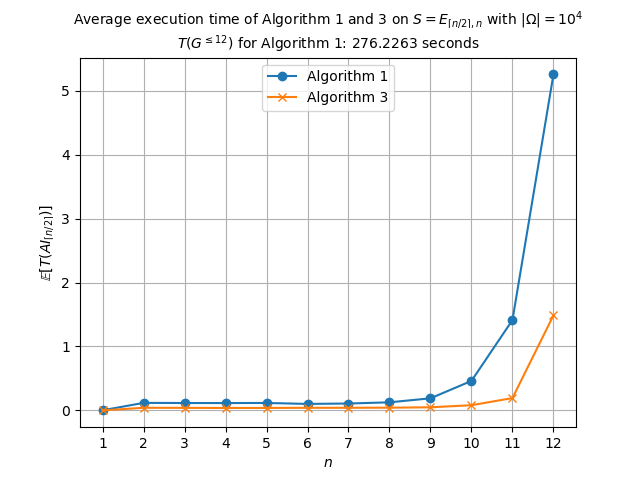
\includegraphics[width=0.7\textwidth]{images/plot_12_10000.png}
    \caption{Average time execution per number of variables of Algorithms~\ref{alg:RMApproach} and \ref{alg:fullAlg3ForAIRestrictesSetOpt} over $10^4$ random $\WAPB{n}$ functions on the set $E_{\lceil{n/2}\rceil,n}$. 
    $T\left(G^{\leq 12}\right)$ gives the time of the pre-computation of the sequence of all Reed-Muller matrices up to $G_{12,12}$.}\label{fig:compTimePlot}
\end{figure}

The pre-computation times of $G^{\leq n_{max}}$ for Algorithm~\ref{alg:RMApproach} are given in the Table~\ref{table:preComputationTimes}. From Figure~\ref{fig:compTimePlot}, we observe that Algorithm~\ref{alg:fullAlg3ForAIRestrictesSetOpt} outperforms Algorithm~\ref{alg:RMApproach} for $n \leq 12$, even without considering the pre-computation time required for $G^{\leq n_{max}}$ and $D^{\leq n_{max}}$ in Algorithm~\ref{alg:RMApproach}. Furthermore, Algorithm~\ref{alg:RMApproach} becomes impractical for $n > 12$ due to the excessive complexity of pre-computation. In contrast, Algorithm~\ref{alg:fullAlg3ForAIRestrictesSetOpt} remains feasible for larger values of $n$. \\
\begin{table}[H]
\centering
\renewcommand{\tabcolsep}{2pt}	
\begin{tabular}{|c|c|c|c|c|c|c|c|c|c|c|c|}
%\toprule
\hline
    $G^{\leq 1}$  & $G^{\leq 2}$  &$G^{\leq 3}$  & $G^{\leq 4}$  & $G^{\leq 5}$  & $G^{\leq 6}$  & $G^{\leq 7}$  &$G^{\leq 8}$ & $G^{\leq 9}$ & $G^{\leq 10}$ & $G^{\leq 11}$  & $G^{\leq 12}$ \\
 %   \midrule
 \hline
     0.0126 & 0.0042 & 0.0017 & 0.004 & 0.0149 & 0.0470 & 0.1938 & 0.806& 3.5456& 14.9168& 65.5014 & 276.2263\\
%     \bottomrule
\hline
\end{tabular}
\caption{Pre-computation time (in seconds) for $G^{\leq n_{max}}$ for $n_{max}$ from $1$ to $12$.}\label{table:preComputationTimes}
\end{table}

Both implementations of the algorithms used to generate the plot in Figure~\ref{fig:compTimePlot} have been developed in \textit{Python}, with the following enhancements:
\begin{itemize}
\item The linear algebra operations in Algorithm~\ref{alg:RMApproach} are performed using the \textit{SageMath} library, while those in Algorithm~\ref{alg:fullAlg3ForAIRestrictesSetOpt} are executed using an ad-hoc custom \textit{Python} package implemented in \textit{Rust}. This setup ensures comparability between the two implementations, as the \textit{SageMath} library is highly optimized for linear algebra operations.
\item The computation of $G^{\leq n_{max}}$ for Algorithm~\ref{alg:RMApproach} is performed using the \textit{generator\_matrix} method of the \textit{SageMath} object \textit{BinaryReedMullerCodes}. While this computation could be more efficient if implemented in \textit{Rust}, the current overall implementation still faces scalability issues. Specifically, for $n \geq 16$, the algorithm becomes impractical because $G_{16,16}$ cannot be stored in a native \textit{Python} list or a \textit{SageMath} matrix object. However, if the entire algorithm were implemented in \textit{Rust}, it could potentially be feasible. Consequently, for larger values of $n$, Algorithm~\ref{alg:RMApproach} is not usable, while Algorithm~\ref{alg:fullAlg3ForAIRestrictesSetOpt} remains viable.
\end{itemize}


\FloatBarrier
\subsection{Determination of $\AIk{k}$ distribution of WPB functions}\label{subsec:AIkWPB}
%Similarly to what has been done in~\cite{Latin:GinMea23} for the weightwise non-linearity $NL_k$, we determine the discrete probability distribution of the $\AIk{k}$ of weightwise perfectly balanced Boolean functions, describing the probability of a function $f\in \WPB{m}$ of having a certain algebraic immunity restricted on the slice $\Ekn{k}{n}$. A more formal definition in given Definition~\ref{def:distAIk} below



Similar to the approach in~\cite{Latin:GinMea23} for analyzing the weightwise nonlinearity $\NLk{k}$, we determine the discrete probability distribution of $\AIk{k}$ for weightwise perfectly balanced Boolean functions. 
This distribution describes the probability that a function $f \in \WPB{m}$ has a specific algebraic immunity restricted to the slice $\Ekn{k}{n}$. 
A formal definition is provided in Definition~\ref{def:distAIk}:

\begin{definition}\label{def:distAIk}
    Let $m \in \N^*$, $n = 2^m$ and $k \in [1,n-1]$, we define the discrete probability distribution of $\AIk{k}$ as:
    \begin{align*}
        p_{\AIk{k}}(x) = \frac{\bigg|\{f\in \WPB{m}\  |\  \AIk{k}(f) = x\}\bigg|}{|\WPB{m}|}.
    \end{align*}
\end{definition}

We aim to determine this distribution for $m = 2, 3$, and $4$. 
However, the number of WPB functions increases fast with the growth of $m$, making this computation infeasible for $m > 2$. In fact, as stated in ~\cite{Latin:GinMea23}, $|\WPB{2}| = 720$, while $|\WPB{3}| > 2^{243}$ and $|\WPB{4}| > 2^{65452}$.\\
Therefore, we have to take a different approach for $m > 2$ by generating a certain number of samples from the set $\WPB{m}$ and calculating the probability over it. The larger the sample size we select, the better we approximate the distribution.

\begin{definition}
    We define the $\AIk{k}$ distribution over a sample $\Omega$ as:
    \begin{align*}
        p_{\Omega,\AIk{k} }(x) =  \frac{\bigg|\{f\in \Omega\ | \  \AIk{k}(f) = x\}\bigg|}{|\Omega|}.
    \end{align*}
\end{definition}


\subsubsection{Determination of the full distribution for \texorpdfstring{m=2}{m=2}}
For $m=2 \Rightarrow n = 4$, it is possible to determine the full probability distribution from Definition~\ref{def:distAIk} without using the random sampling strategy. 
The resulting plots can be found on Figure~\ref{fig:dullDist} and Figure~\ref{fig:averagesFullDist} while the corresponding probability distribution table is presented in Table~\ref{table:probabilityDistributionn4}. 

\begin{figure}[ht]
    \centering
    \begin{minipage}[b]{0.45\textwidth}
        \centering
        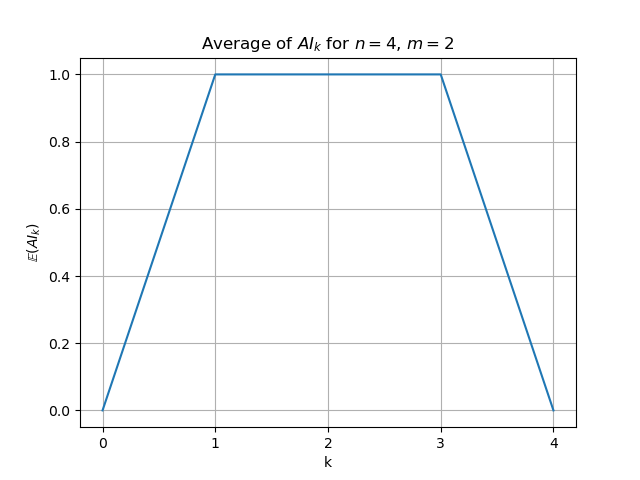
\includegraphics[width=\textwidth]{images/WPB_2_sample_size_full_dist.png}
        \caption{Mean of $\AIk{k}$ over $\WPB{2}$.}
        \label{fig:averagesFullDist}
    \end{minipage}
    \hfill
    \begin{minipage}[b]{0.5\textwidth}
        \centering
        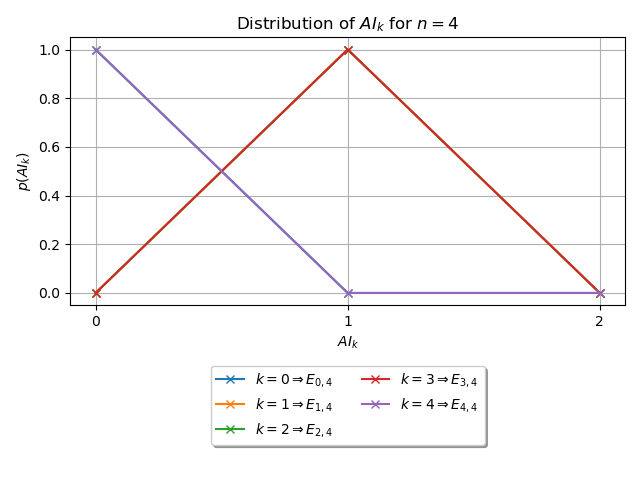
\includegraphics[width=\textwidth]{images/WPB_2_sample_size_full_dist_prob.png}
        \caption{Probability distribution of $\AIk{k}$  over $\WPB{2}$.}
        \label{fig:probFullDist}
    \end{minipage}
    \caption{Mean of $\AIk{k}$ and probability distribution of $\AIk{k}$ from Definition~\ref{def:distAIk} of $4$-variable WPB functions.}
    \label{fig:dullDist}
\end{figure}

\subsubsection{Random Sampling}
In practice, random sampling is performed by generating a set $\Omega_k = \{\omega_1^{(k)}, \cdots, \omega_{|\Omega|}^{(k)}\}$ consisting of $|\Omega|$ random balanced sub-truth tables for each slice $\Ekn{k}{n}$. 
Then, for each slice $\Ekn{k}{n}$, the $\AIk{k}$ is computed for each restricted set in $\Omega_k$ the frequency of each particular $\AIk{k}$ value is recorded.
Depending on the value of $m$ and the chosen sample size, the number of sub-truth tables generated may be too large to fit in memory simultaneously. 
To address this, it is crucial to avoid storing all elements in memory at once. 
Instead, they should be processed one by one, either by computing sequentially or by using iterators.\\
The following procedure is done for each slice $\Ekn{k}{n}$:
\begin{enumerate}
    \item Initialize a hash table of all possible values of $\AIk{k}$.
    \item For each sub-truth table in $\omega_i^{(k)} \in \Omega_k$ (note that $\omega_i^{(k)}$ is either generated on the fly by an iterator or by having the source code for the generation of $\omega_i^{(k)}$ in this loop)\footnotemark:
    \begin{enumerate}
        \item Run Algorithm~\ref{alg:fullAlg3ForAIRestrictesSetOpt} with $S=\omega_i^{(k)}$\label{enum:stepOfapplicationEnum}.
        \item Increment the value in the hash table corresponding to the output of the previous step.
    \end{enumerate}
    \item Divide each value in the hash table by $|\Omega|$.
\end{enumerate}

\noindent
\textbf{Results for $n=8$ and sample size$=2^{15}$}.
Figure~\ref{fig:probDist32768} represents the $\AIk{k}$ distribution, Table~\ref{table:probabilityDistributionn8} shows the corresponding values, and Figure~\ref{fig:averages32768} the average values.
We observe that for $n=4$ all WPB functions have the same values of $\AIk{k}$, for every $k$. 
However, for $n=8$, there are WPB functions with different restricted $\AIk{k}$, for example with $k=4$ we observe functions reaching the lowest value ($2$, such as families exhibited in~\cite{Latin:GinMea23}) and some reaching $3$ which is optimal for this size.
\begin{figure}[H]
    \centering
    \begin{minipage}[b]{0.45\textwidth}
        \centering
        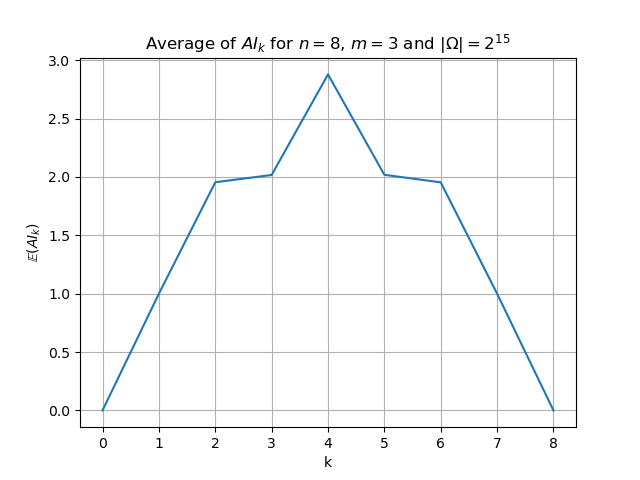
\includegraphics[width=\textwidth]{images/WPB_3_sample_size_32768_average_a.png}
        \caption{Estimated average of $\AIk{k}$ over $\WPB{3}$.}
        \label{fig:averages32768}
    \end{minipage}
    \hfill
    \begin{minipage}[b]{0.5\textwidth}
        \centering
        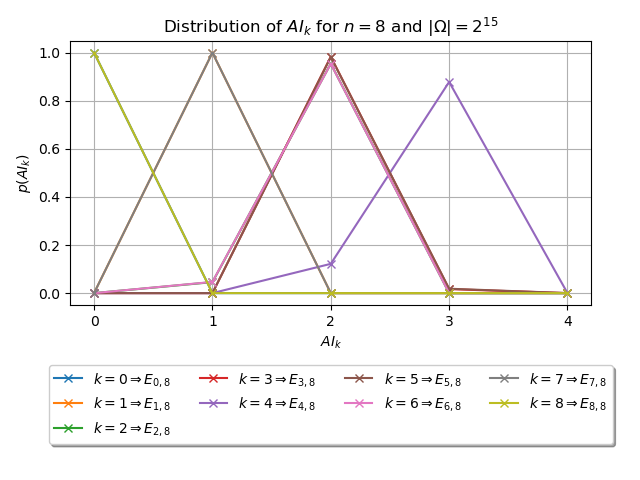
\includegraphics[width=\textwidth]{images/WPB_3_sample_size_32768_dist_prob_a.png}
        \caption{Estimated Probability distribution of $\AIk{k}$ over $\WPB{3}$.}
        \label{fig:probDist32768}
    \end{minipage}
    \caption{Estimated average of $\AIk{k}$ and probability distribution of $\AIk{k}$ over $8$-variable WPB functions, with $2^{15}$ samples.}
    \label{fig:main2}
\end{figure}

%\noindent
%\pmnote{results for n=16 here also as for 8+ some remarks

%@ Luca, do you have a table version of Figure 9? I do not manage to identify the curve to give observations.}\\
%\lbnote{Tables added in Table~\ref{table:probability_distributions}.}

\textbf{Results for $n=16$ and sample size$=2^{10}$}.
Figure~\ref{fig:probDist2014} represents the $\AIk{k}$ distribution, Table~\ref{table:probabilityDistributionn16} shows the corresponding values and Figure~\ref{fig:averages2014} the average values.
We observe that there are WPB functions with different restricted $\AIk{k}$ for this value of $n$, and that for the central values ok $k$, all functions we sampled reach the optimal value of $\AIk{k}$.

The average execution times for the $\AIk{k}$ distributions with $n=4$, $n=8$ are $n=16$ are displayed in Tables~\ref{table:averagesFullDist},~\ref{table:averages32768} and~\ref{table:averages16VarsSampleSize1024}.

%is already enough variability in the corpus of WPB functions to observe 

\footnotetext[10]{Step $2$ may be executed in parallel on the $\omega_i^{(k)}$s.}

%\pmnote{add some comment on the results in 4 and 8 variables.}
\begin{figure}[H]
    \centering
    \begin{minipage}[b]{0.45\textwidth}
        \centering
        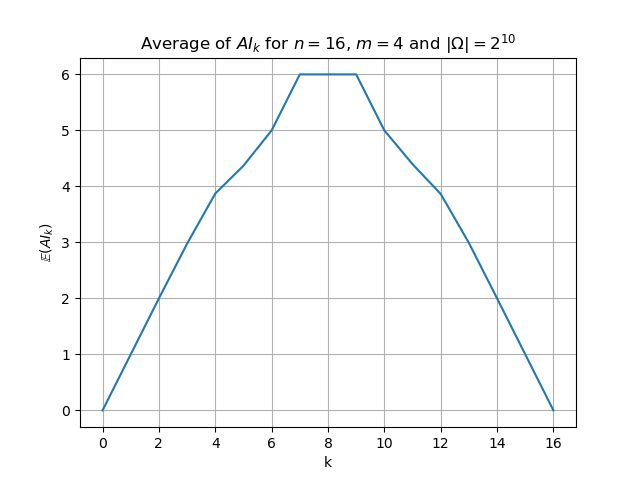
\includegraphics[width=\textwidth]{images/WPB_4_sample_size_1024_average_a.png}
        \caption{Estimated average of $\AIk{k}$ over $\WPB{4}$.}
        \label{fig:averages2014}
    \end{minipage}
    \hfill
    \begin{minipage}[b]{0.5\textwidth}
        \centering
        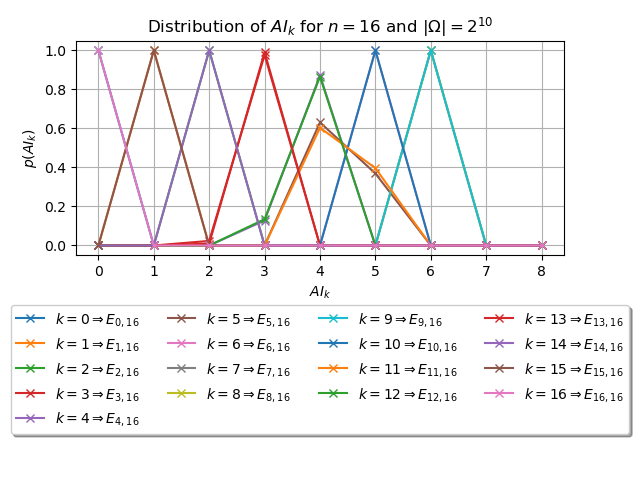
\includegraphics[width=\textwidth]{images/WPB_4_sample_size_1024_dist_prob_a.png}
        \caption{Estimated Probability distribution of $\AIk{k}$ over $\WPB{4}$.}
        \label{fig:probDist2014}
    \end{minipage}
    \caption{Estimated average of $\AIk{k}$ and probability distribution of $\AIk{k}$ over $8$-variable WPB functions, with $2^{10}$ samples.}
    \label{fig:main2014}
\end{figure}


\begin{table}[H]
    \centering
    \caption{$\AIk{k}$ probability distribution of $\WPB{2}$, $\WPB{3}$ and $\WPB{4}$.}
    \label{table:probability_distributions}
    
    \begin{subtable}[t]{0.4\textwidth}
        \centering
        \caption{Probability distribution $p_{\AIk{k}}$ for $n=4$, $m=2$.}
        \label{table:probabilityDistributionn4}
        \renewcommand{\arraystretch}{1.2} % Improve readability
    \renewcommand{\tabcolsep}{2pt}	
    \begin{tabular}{r|rrrrr}
    	\toprule
    	$p(x)$, $k$ & 0 & 1 & 2 & 3 & 4 \\
    	\midrule
    	0 & 1.00 & 0.00 & 0.00 & 0.00 & 1.00 \\
    	1 & 0.00 & 1.00 & 0.00 & 1.00 & 0.00 \\
    	2 & 0.00 & 0.00 & 1.00 & 0.00 & 0.00 \\
    	\bottomrule
    \end{tabular}
    \end{subtable}%
    \hfill
    \begin{subtable}[t]{0.55\textwidth}
        \centering
        \caption{Probability distribution $p_{\Omega, \AIk{k}}$ for $n=8$, $m=3$, $\Omega = 2^{15}$.}
        \label{table:probabilityDistributionn8}
        \renewcommand{\arraystretch}{1.2}

\renewcommand{\tabcolsep}{2pt}	
\begin{tabular}{r|rrrrrrrrr}
	\toprule
	$p(x)$, $k$ & 0 & 1 & 2 & 3 & 4 & 5 & 6 & 7 & 8 \\
	\midrule
	0 & 1.00 & 0.00 & 0.00 & 0.00 & 0.00 & 0.00 & 0.00 & 0.00 & 1.00 \\
	1 & 0.00 & 1.00 & 0.00 & 0.00 & 0.00 & 0.00 & 0.05 & 1.00 & 0.00 \\
	2 & 0.00 & 0.00 & 1.00 & 0.98 & 0.00 & 0.98 & 0.95 & 0.00 & 0.00 \\
	3 & 0.00 & 0.00 & 0.00 & 0.02 & 0.13 & 0.02 & 0.00 & 0.00 & 0.00 \\
	4 & 0.00 & 0.00 & 0.00 & 0.00 & 0.87 & 0.00 & 0.00 & 0.00 & 0.00 \\
	\bottomrule
\end{tabular}    
    \end{subtable}

    \vspace{1em} % Add some space between rows of tables

    \begin{subtable}[t]{1\textwidth}
        \centering
        \caption{Probability distribution $p_{\Omega, \AIk{k}}$ for $n=16$, $m=4$, $\Omega = 2^{10}$.}
        \label{table:probabilityDistributionn16}
        \renewcommand{\arraystretch}{1.2}


 \resizebox{\textwidth}{!}{
 \renewcommand{\tabcolsep}{2pt}	
 \begin{tabular}{r|rrrrrrrrrrrrrrrrr}
 	\toprule
 	$p(x)$, $k$ & 0  & 1  & 2  & 3  & 4  & 5  & 6  & 7  & 8  & 9  & 10 & 11 & 12 & 13 & 14 & 15 & 16 \\
 	\midrule
 	0  & 1.00 & 0.00 & 0.00 & 0.00 & 0.00 & 0.00 & 0.00 & 0.00 & 0.00 & 0.00 & 0.00 & 0.00 & 0.00 & 0.00 & 0.00 & 0.00 & 1.00 \\
 	1  & 0.00 & 1.00 & 0.00 & 0.00 & 0.00 & 0.00 & 0.00 & 0.00 & 0.00 & 0.00 & 0.00 & 0.00 & 0.00 & 0.00 & 0.00 & 1.00 & 0.00 \\
 	2  & 0.00 & 0.00 & 1.00 & 0.02 & 0.00 & 0.00 & 0.00 & 0.00 & 0.00 & 0.00 & 0.00 & 0.00 & 0.00 & 0.01 & 1.00 & 0.00 & 0.00 \\
 	3  & 0.00 & 0.00 & 0.00 & 0.98 & 0.13 & 0.00 & 0.00 & 0.00 & 0.00 & 0.00 & 0.00 & 0.00 & 0.13 & 0.99 & 0.00 & 0.00 & 0.00 \\
 	4  & 0.00 & 0.00 & 0.00 & 0.00 & 0.87 & 0.63 & 0.00 & 0.00 & 0.00 & 0.00 & 0.00 & 0.60 & 0.87 & 0.00 & 0.00 & 0.00 & 0.00 \\
 	5  & 0.00 & 0.00 & 0.00 & 0.00 & 0.00 & 0.37 & 1.00 & 0.00 & 0.00 & 0.00 & 1.00 & 0.40 & 0.00 & 0.00 & 0.00 & 0.00 & 0.00 \\
 	6  & 0.00 & 0.00 & 0.00 & 0.00 & 0.00 & 0.00 & 0.00 & 1.00 & 1.00 & 1.00 & 0.00 & 0.00 & 0.00 & 0.00 & 0.00 & 0.00 & 0.00 \\
 	\bottomrule
 \end{tabular}
 }
 
 
    \end{subtable}

\end{table}

\begin{table}[H]
    \centering
    \caption{Averages execution times and $\AI{k}$ of $\WPB{2}$, $\WPB{3}$ and $\WPB{4}$ functions.}
    \label{table:transposed_averages}

    \begin{subtable}[t]{0.8\textwidth}
        \centering
        \caption{Average execution time and $\AIk{k}$ for $n=4$, $m=2$.}
        \label{table:averagesFullDist}
        \renewcommand{\arraystretch}{1.2}
        \renewcommand{\tabcolsep}{3pt}	
        \begin{tabular}{r|ccccc}
            \toprule
            $k$ & 0 & 1 & 2 & 3 & 4 \\
            \midrule
            $\mathbb{E}[T(AI_k)]$ & $0.53\times 10^{-4}$ & $0.0526$ & $0.0487$ & $0.0586$ & $0.6\times10^{-5}$\\
            $\mathbb{E}[AI_k]$     & $0.00$     & $1.00$     & $1.00$     & $1.00$     & $0.00$ \\
            \bottomrule
        \end{tabular}
    \end{subtable}

    \vspace{1em} % Add space between tables

    \begin{subtable}[t]{0.9\textwidth}
        \centering
        \caption{Average execution time and $\AIk{k}$ for $n=8$, $m=3$ and $\mbox{sampleSize}=2^{15}$.}
        \label{table:averages32768}
        \renewcommand{\arraystretch}{1.2}
        \resizebox{\textwidth}{!}{ % Resize to fit within page width
        \renewcommand{\tabcolsep}{3pt}	
        \begin{tabular}{r|ccccccccc}
            \toprule
            $k$ & 1 & 2 & 3 & 4 & 5 & 6 & 7\\
            \midrule
            $\mathbb{E}[T(AI_k)]$ & $0.0756$ & $0.086$ & $0.094$ & $0.090$ & $0.102$ & $0.092$ & $0.0938$ \\
            $\mathbb{E}[AI_k]$  & $1.00$     & $1.95$     & $2.02$     & $2.89$     & $2.02$     & $1.95$     & $1.00$     \\
            \bottomrule
        \end{tabular}
        }
    \end{subtable}

    \vspace{1em} % Add space between tables

    \begin{subtable}[t]{1.1\textwidth}
        \centering
        \caption{Average execution time and $\AIk{k}$ for $n=16$, $m=4$ and $\mbox{sampleSize}=2^{10}$.}
        \label{table:averages16VarsSampleSize1024}
        %\renewcommand{\arraystretch}{1.2}
        \resizebox{\textwidth}{!}{ % Resize to fit within page width
        \renewcommand{\tabcolsep}{2pt}	
        \begin{tabular}{r|cccccccccccccccccc}
            \toprule
            $k$ & 1 & 2 & 3 & 4 & 5 & 6 & 7 & 8 & 9 & 10 & 11 & 12 & 13 & 14 & 15\\
            \midrule
            $\mathbb{E}[T(AI_k)]$ & $0.334$ & $0.342$ & $0.41$ & $4.01$ & $91.81$ & $636.37$ & $2838.92$ & $6384.38$ & $3111.12$ & $732.50$ & $118.96$ & $5.23$ & $0.43$ & $0.35$ & $0.35$\\
            $\mathbb{E}[AI_k]$ & $1.00$     & $2.00$     & $2.98$     & $3.87$     & $4.37$     & $5.00$     & $6.00$     & $6.00$     & $6.00$     & $5.00$     & $4.40$     & $3.87$     & $2.99$     & $2.00$     & $1.00$\\
            \bottomrule
        \end{tabular}
        }
    \end{subtable}
\end{table}

\begin{comment}
\begin{table}[H]
    \centering
\begin{minipage}{0.45\textwidth}
    \centering
    \begin{tabular}{|c|c|c|}%{rrr}
 %       \toprule
 \hline
        $k$ &  $\mathbb{E}[T(AI_k)]$ &  $\mathbb{E}[AI_k]$ \\ \hline
%        \midrule
        0 &               $0.000053$ &                 0.0 \\ \hline
        1 &               $0.052649$ &                 1.0 \\ \hline
        2 &               $0.048703$ &                 1.0 \\\hline
        3 &               $0.058630$ &                 1.0 \\\hline
        4 &               $0.000006$ &                 0.0 \\ \hline
  %      \bottomrule
    \end{tabular}
    \caption{Average execution time and $\AIk{k}$ for $n=4$, $m=2$}
    \label{table:averagesFullDist}
\end{minipage}
\hfill
\begin{minipage}{0.45\textwidth}
        \centering
        \begin{tabular}{|c|c|c|}%{rrr}
%\toprule
\hline
 $k$ &  $\mathbb{E}[T(AI_k)]$ &  $\mathbb{E}[AI_k]$ \\ \hline
%\midrule
   0 &               $4.768372 * 10^{-6}$ &            $0.00$ \\ \hline
   1 &               $0.075641$ &            $1.00$ \\ \hline
   2 &               $0.086194$ &            $1.95$ \\ \hline
   3 &               $0.094307$ &            $2.02$ \\ \hline
   4 &               $0.089607$ &            $2.89$ \\ \hline
   5 &               $0.101818$ &            $2.02$ \\ \hline
   6 &               $0.092377$ &            $1.95$ \\ \hline
   7 &               $0.093818$ &            $1.00$ \\ \hline
   8 &               $1.621246 * 10^{-5}$ &            $0.00$ \\ \hline
%\bottomrule
\end{tabular}
        \caption{Average execution time and $\AIk{k}$ for $n=8$, $m=3$ and $\mbox{sampleSize}=2^{15}$}
        \label{table:averages32768}
    \end{minipage}
\begin{minipage}{0.45\textwidth}
        \centering
        \begin{tabular}{|c|c|c|}%{rrr}
%\toprule
\hline
 $k$ &  $\mathbb{E}[T(AI_k)]$ &  $\mathbb{E}[AI_k]$ \\ \hline
%\midrule
   0 & $0.000010$ & $0.00$\\ \hline
   1 & $0.334046$ & $1.00$\\ \hline
   2 & $0.342011$ & $2.00$\\ \hline
   3 & $0.408244$ & $2.98$\\ \hline
   4 & $4.011003$ & $3.87$\\ \hline
   5 & $91.810299$ & $4.37$\\ \hline
   6 & $636.368421$ & $5.00$\\ \hline
   7 & $2838.922261$ & $6.00$\\ \hline
   8 & $6384.383319$ & $6.00$\\ \hline
   9 & $3111.118973$ & $6.00$\\ \hline
   10 & $732.501775$ & $5.00$ \\ \hline
   11 & $118.963582$ & $4.40$\\ \hline
   12 & $5.229858$ & $3.87$ \\ \hline
   13 & $0.426482$ & $2.99$\\ \hline
   14 & $0.353760$ & $2.00$ \\ \hline
   15 & $0.344984$ & $1.00$ \\ \hline
   16 & $0.000015$ & $0.00$ \\ \hline
%\bottomrule
\end{tabular}
        \caption{Average execution time and $\AIk{k}$ for $n=16$, $m=4$ and $\mbox{sampleSize}=2^{10}$}
        \label{table:averages16VarsSampleSize1024}
    \end{minipage}
\end{table}
\end{comment}

\FloatBarrier
\subsection{Determination of $\AIk{k}$ of known WPB families}\label{subsec:AIkknownFam}
In this part, we determine the $\AIk{k}$s of functions introduced in~\cite{Mat:ZJZQ23},~\cite{AMC:DalMal23},~\cite{CC:TangLiu19} and in~\cite{TOSC:CarMeaRot17} for $n=8$ and $16$ variables.

The results are summarized in Table~\ref{table:publiedFunctions}. 
Of the four WPB calculations we performed, the one in ~\cite{CC:TangLiu19} is the one that would resist the best to algebraic attacks (with constant Hamming weight inputs), as it achieves higher $\AIk{k}$ values for both $n = 8$ and $ n = 16$. In contrast, the one in~\cite{Mat:ZJZQ23}, would be the least resistant, as it has the overall lower $\AIk{k}$ for both $n=8$ and $n=16$. Specifically:
\begin{itemize}
\item $n=8$. 
The function in~\cite{Mat:ZJZQ23} has a constant $\AIk{k}$ of $2$ for $k \in [2, 6]$ and the functions in~\cite{TOSC:CarMeaRot17} a constant $\AIk{k}$ of $2$ for $k \in [3, 6]$, whereas the functions in~\cite{AMC:DalMal23} and in~\cite{CC:TangLiu19} achieve an $\AIk{4}$ of $3$.

\item $n=16$. 
The function in~\cite{Mat:ZJZQ23} again has a constant $\AIk{k}$ of $2$ for $k \in [2, 14]$. 
In contrast, the function in~\cite{CC:TangLiu19} achieves an $\AIk{k}$ of $3$ for $k = 4,5,11$ and $12$, an $\AIk{k}$ of $4$ for $k = 6,7,9$ and $10$ and an $\AIk{k}$ of $5$ for $k=8$. The functions~\cite{AMC:DalMal23} and in~\cite{TOSC:CarMeaRot17}, both reach an $\AIk{k}$ of $3$ but for $k\in [4,12]$ and $k\in [5,13]$ respectively.
\end{itemize}

%Table~\ref{table:publiedFunctions} shows these results. 
%We see that~\cite{AMC:DalMal23} is more secure than~\cite{Mat:ZJZQ23} since it has a better $\AIk{k}$s for both $n=8$ and $n=16$. In particular
%\begin{description}
%	\item[n=8] ~\cite{Mat:ZJZQ23} has a constant $AI_k$ of $2$ for $k\in [2,7]$, while ~\cite{AMC:DalMal23} has a $AI_k$ of $3$ for $k=5$
%	\item[n=16] ~\cite{Mat:ZJZQ23} has a constant $AI_k$ of $2$, $k\in [2,14]$, while ~\cite{AMC:DalMal23} has a $AI_k$ of $3$ for $k=5,7,9$ and $11$.
%\end{description}

The maximum execution times for~\cite{AMC:DalMal23}, ~\cite{Mat:ZJZQ23},~\cite{CC:TangLiu19} and~\cite{TOSC:CarMeaRot17} with $n=8$ occur with $k=4$ and are around $0.014$, $0.029$, $0.011$ and $0.012$ seconds, respectively.\\
% LT19 k=8 time = 126.627561
% ZS k=8 time = 5.898671
% DM24 k = 9 time = 7.935819
% CMR k = 8 time = 12.048051
For $n=16$, the maximum execution times for~\cite{Mat:ZJZQ23},~\cite{CC:TangLiu19} and ~\cite{TOSC:CarMeaRot17} occur with $k=8$ and are $5.898671$, $126.627561$ and $12.048051$ seconds respectively. In contrast, for~\cite{AMC:DalMal23}, the maximum execution time occurs for $k=9$ and is $7.935819$ seconds.

\begin{table}[H]
\center
%\renewcommand{\tabcolsep}{0.5pt}	
\caption{$\AIk{k}$ of the construction from~\cite{AMC:DalMal23}, from~\cite{Mat:ZJZQ23}, from~\cite{CC:TangLiu19} and from~\cite{TOSC:CarMeaRot17} with $m=3$ ($n=8$) and $m=4$ ($n=16$).\label{table:publiedFunctions}}
%\resizebox{\textwidth}{!}{
\renewcommand{\tabcolsep}{3pt}	
\begin{tabular}{|c|c|c|c|c|c|c|c|c|c|c|c|c|c|c|c|c|c|}
\hline
\multicolumn{18}{|c|}{~\cite{AMC:DalMal23}} \\
\hline
$n$, $k$ & $0$ & $1$ & $2$ & $3$ & $4$ & $5$ & $6$ & $7$ & $8$ & $9$ & $10$ & $11$ & $12$ & $13$ & $14$ & $15$ & $16$ \\
\hline
8 & 0 & 1 & 1 & 2 & 3 & 2 & 2 & 1 & 0 &  &  &  &  &  &  &  &  \\
16 & 0 & 1 & 1 & 2 & 3 & 3 & 3 & 3 & 3 &  3 & 3 & 3 & 3 & 2 & 2 & 1 & 0 \\
\hline
\multicolumn{18}{|c|}{~\cite{Mat:ZJZQ23}} \\
\hline
$n$, $k$ & $0$ & $1$ & $2$ & $3$ & $4$ & $5$ & $6$ & $7$ & $8$ & $9$ & $10$ & $11$ & $12$ & $13$ & $14$ & $15$ & $16$ \\
\hline
8 & 0 & 1 & 2 & 2 & 2 & 2 & 2 & 1 & 0 &  &  &  &  &  &  &  &  \\
16 & 0 & 1 & 2 & 2 & 2 & 2 & 2 & 2 & 2 & 2  & 2 & 2 & 2 & 2 & 2 & 1 & 0 \\
\hline
\multicolumn{18}{|c|}{~\cite{CC:TangLiu19}} \\
\hline
$n$, $k$ & $0$ & $1$ & $2$ & $3$ & $4$ & $5$ & $6$ & $7$ & $8$ & $9$ & $10$ & $11$ & $12$ & $13$ & $14$ & $15$ & $16$ \\
\hline
8 & 0 & 1 & 2 & 2 & 3 & 2 & 2 & 1 & 0 &  &  &  &  &  &  &  &  \\
16 & 0 & 1 & 2 & 2 & 3 & 3 & 4 & 4 & 5 & 4  & 4 & 3 & 3 & 2 & 2 & 1 & 0 \\
\hline
\multicolumn{18}{|c|}{~\cite{TOSC:CarMeaRot17}} \\
\hline
$n$, $k$ & $0$ & $1$ & $2$ & $3$ & $4$ & $5$ & $6$ & $7$ & $8$ & $9$ & $10$ & $11$ & $12$ & $13$ & $14$ & $15$ & $16$ \\
\hline
8 & 0 & 1 & 1 & 2 & 2 & 2 & 2 & 1 & 0 &  &  &  &  &  &  &  &  \\
16 & 0 & 1 & 1 & 2 & 2 & 3 & 3 & 3 & 3 & 3  & 3 & 3 & 3 & 3 & 2 & 1 & 0 \\
\hline
\end{tabular}
\end{table}


In Table~\ref{tab:WPB8}, we summarize the results on $\AIk{k}$ for WPB functions with $8$ variables, including both our findings and those from the state of the art.  
Similarly, Table~\ref{tab:WPB16} presents the corresponding results for functions with $16$ variables.  
We observe that most of the studied families exhibit lower weightwise algebraic immunity than a randomly chosen WPB function, with the exception of the field order construction~\cite{eprint:Meaux24}.  


\begin{table}[H]
	\center 
	\renewcommand{\tabcolsep}{1.8pt}	
	\begin{tabular}{|c| c|c|c|c|c|}
		\hline
		Function &  $\AIk{2}$ & $\AIk{3}$ & $\AIk{4}$ &  $\AIk{5}$ & $\AIk{6}$  \\ \hline 
		\cite{AMC:DalMal23} & $1$ &  $2$ & $2$  &  $2$ & $1$ \\ \hline
		\cite{Mat:ZJZQ23} & $2$ &  $2$ & $2$  &  $2$ & $2$ \\ \hline
        \cite{CC:TangLiu19} & $2$ &  $2$ & $3$  &  $2$ & $2$ \\ \hline
        \cite{TOSC:CarMeaRot17} & $1$ &  $2$ & $2$  &  $2$ & $2$ \\ \hline
		Estimated average & $1.95$ &  $2.02$ & $2.87$  &  $2.02$ & $1.95$ \\ \hline
		Field order~\cite{eprint:Meaux24} &$ 1$& $2$& $3$& $2$ &$2$ \\	\hline
		Upper bound & $2$ &  $3$ & $3$  &  $3$ & $2$ \\	\hline
	
		
	\end{tabular}
	\caption{$\AIk{k}$ of WPB functions in $8$ variables.}
	\label{tab:WPB8}
\end{table}


\begin{table}[H]
	\centering 
    \resizebox{\textwidth}{!}{
	\renewcommand{\tabcolsep}{1.8pt}	
	\begin{tabular}{|c| c|c|c|c|c| c|c|c|c|c| c|c|c| }
		\hline
		Function &  $\AIk{2}$ & $\AIk{3}$ & $\AIk{4}$ &  $\AIk{5}$ & $\AIk{6}$ &  $\AIk{7}$ & $\AIk{8}$ & $\AIk{9}$ &  $\AIk{10}$ & $\AIk{11}$ &  $\AIk{12}$ & $\AIk{13}$ & $\AIk{14}$ \\ \hline 
		
\cite{AMC:DalMal23}		&$ 1$& $2$& $3$& $3$ &$3$ & $3$ &$3$ &$3$ &$3$ &$3$ &$2$ &$2$
	 &0 \\ \hline
\cite{Mat:ZJZQ23}		&$ 2$& $2$& $2$& $2$ &$2$ & $2$ &$2$ &$2$ &$2$ &$2$ &$2$ &$2$
&$2$ \\ \hline
\cite{CC:TangLiu19}		&$ 2$& $2$& $3$& $3$ &$4$ & $4$ &$5$ &$4$ &$4$ &$3$ &$3$ &$2$
&$2$ \\ \hline	
\cite{TOSC:CarMeaRot17}		&$1$& $2$& $2$& $3$ &$3$ & $3$ &$3$ &$3$ &$3$ &$3$ &$3$ &$3$
&$2$ \\ \hline	
		Estimated average &$2.00$& $2.99$& $3.89$& $4.37$ &$5.00$ & $6.00$ &$6.00$ &$6.00$ &5.00 &$4.40$ &$3.87$ &$2.99$ &$2.00$ \\ \hline
%2 3 4 4 5 6 6 6 5 4 3 2 2		
		Field order~\cite{eprint:Meaux24} &$ 2$& $3$& $4$& $4$ &$5$ & $6$ &$6$ &$6$ &$5$ &$4$ &$3$ &$2$ &$2$ \\	\hline
		Upper bound &$ 2$& $3$& $4$& $5$ &$5$ & $6$ &$6$ &$6$ &$5$ &$5$ &$4$ &$3$ &$2$  \\	\hline
		
		
	\end{tabular}
    }
	\caption{$\AIk{k}$ of WPB functions in $16$ variables.}
	\label{tab:WPB16}
\end{table}

%\section{Conclusion and open questions}
\section{Conclusion}


%In this article we formalized the main theoretical arguments and provided the algorithms to compute the restricted algebraic immunity over any set $S \subset \F_2^n$, using the Reed-Muller and the iterative approach.
%We compared the complexity of our algorithms in practice, and showed the iterative approach is more performant. Then, we used our results to compute or estimate for the first time the distribution of the $\AI_k$ of WPB functions in $4$, $8$ and $16$ variables. 
%Moreover we determined the $\AI_k$ of various family of WPB functions exhibited in former works, and show that most of them perform worse than a random WPB function relatively to this parameter.

%We hope formalizing the theoretical background and providing algorithms and implementations for the computation of the restricted algebraic immunity will be useful for further research and implementation of variants of the algebraic attack. 


In this article, we formalized the main theoretical foundations and provided algorithms for computing restricted algebraic immunity over any set $S \subseteq \F_2^n$, using both the Reed-Muller and iterative approaches. 
We compared the practical complexity of these algorithms and showed that the iterative approach is more efficient. 
Additionally, we applied our methods to compute or estimate, for the first time, the distribution of $\AI_k$ for WPB functions with $4$, $8$, and $16$ variables. 
Furthermore, we determined the values of $\AI_k$ for various families of WPB functions introduced in previous works and showed that, in most cases, these functions exhibit lower weightwise algebraic immunity than a randomly chosen WPB function.  

By formalizing the theoretical background and providing both algorithms and implementations for computing restricted algebraic immunity, we hope this work will contribute to further research and the practical implementation of algebraic attack variants. 





%\section{Acknowledgments}
%Pierrick Méaux was supported by the ERC Advanced Grant no. 787390.



\newpage

%%%%%%%%%%%%%%%%%%%%%%%%%%%%%%%%%%%%%%%~


\ifnum\full=0
%%%%%%%%%%%%%%%%%%%%%%%%%%%%%%%%%%%%%%%%%%%%
\bibliographystyle{splncs04}
\bibliography{add}
%%%%%%%%%%%%%%%%%%%%%%%%%%%%%%%%%%%%%%%%%%%%
\else
%%%%%%%%%%%%%%%%%%%%%%%%%%%%%%%%%%%%%%%%%%%%
\bibliographystyle{alpha}
\bibliography{add}
%%%%%%%%%%%%%%%%%%%%%%%%%%%%%%%%%%%%%%%%%%%%
\fi

%\newpage
% \appendix


\end{document}

